% the following command is only required if the thesis is written in german
\RequirePackage[ngerman=ngerman-x-latest]{hyphsubst}

\documentclass[
  ngerman, % change to ngerman for german theses
  symmetric, % use two-side for booklike layouts
  numbers=noenddot % remove trailing dots in chapter/section/... enumeration
]{tudscrreprt}

\usepackage[T1]{fontenc}
\usepackage[utf8]{inputenc}
\usepackage[
  ngerman % change to ngerman for german theses
]{babel}
\usepackage{isodate}
\usepackage{pdfpages}
\usepackage{listings}
\usepackage[toc, page]{appendix}
\usepackage{hyphenat}

\usepackage[
  style=alphabetic,
  backend=biber,
  url=false,
  doi=false,
  isbn=false,
  hyperref,
]{biblatex}
% configure the location of the biblatex file
\addbibresource{bibliography.bib}
\AtEveryBibitem{%
  \clearfield{note}%
}

% make all links clickable but hide ugly boxes
\usepackage[hidelinks]{hyperref}
% automatically insert Fig. X in the text with \cref{..}
\usepackage[capitalise,nameinlink,noabbrev]{cleveref}

\usepackage[colorinlistoftodos,prependcaption,textsize=tiny]{todonotes}

\usepackage{graphicx}
\graphicspath{ {./images/} }

\usepackage{svg}

% if you need mathy stuff
\newtheorem{lem}{Lemma}
\crefname{lem}{Lemma}{Lemmas}
\newtheorem{thm}{Theorem}
\crefname{thm}{Theorem}{Theorems}
\newtheorem{defs}{Definition}
\crefname{defs}{Def.}{Defs.}

\usepackage{blindtext}

%\usepackage{tudscrsupervisor} % if you want to copy the sources of the task description into the thesis

\usepackage{csquotes}

\usepackage{caption}
\captionsetup{font=normalfont,labelfont=normalfont,labelsep=space}
\usepackage{floatrow}
\floatsetup{font=normalfont}
\floatsetup[table]{style=plaintop}
\captionsetup{singlelinecheck=off,format=hang,justification=raggedright}
\DeclareCaptionSubType[alph]{figure}
\DeclareCaptionSubType[alph]{table}
\captionsetup[subfloat]{labelformat=brace,list=off}

\usepackage{booktabs}
\usepackage{array}
\usepackage{tabularx}
\usepackage{tabulary}
\usepackage{tabu}
\usepackage{longtable}
\usepackage{multirow}

\usepackage{quoting}

\usepackage[babel]{microtype}

\usepackage{xfrac}

\usepackage{enumitem}
\setlist[itemize]{noitemsep}

\usepackage{ellipsis}
\let\ellipsispunctuation\relax

\usepackage{xcolor, soul}

\colorlet{hlcolor}{lightgray!20}
\sethlcolor{hlcolor}

\DeclareRobustCommand{\texttt}[1]{%
    \hl{\ttfamily#1}%
}

\usepackage{listings}
\usepackage{xcolor}

\definecolor{commentsColor}{rgb}{0.497495, 0.497587, 0.497464}
\definecolor{keywordsColor}{rgb}{0.000000, 0.000000, 0.635294}
\definecolor{stringColor}{rgb}{0.558215, 0.000000, 0.135316}

\lstset{ %
  backgroundcolor=\color{white},   % choose the background color; you must add \usepackage{color} or \usepackage{xcolor}
  basicstyle=\footnotesize,        % the size of the fonts that are used for the code
  breakatwhitespace=false,         % sets if automatic breaks should only happen at whitespace
  breaklines=true,                 % sets automatic line breaking
  captionpos=b,                    % sets the caption-position to bottom
  commentstyle=\color{commentsColor}\textit,    % comment style
  deletekeywords={...},            % if you want to delete keywords from the given language
  escapeinside={\%*}{*)},          % if you want to add LaTeX within your code
  extendedchars=true,              % lets you use non-ASCII characters; for 8-bits encodings only, does not work with UTF-8
  frame=tb,	                   	   % adds a frame around the code
  keepspaces=true,                 % keeps spaces in text, useful for keeping indentation of code (possibly needs columns=flexible)
  keywordstyle=\color{keywordsColor}\bfseries,       % keyword style
  language=Python,                 % the language of the code (can be overrided per snippet)
  otherkeywords={*,...},           % if you want to add more keywords to the set
  numbers=left,                    % where to put the line-numbers; possible values are (none, left, right)
  numbersep=5pt,                   % how far the line-numbers are from the code
  numberstyle=\tiny\color{commentsColor}, % the style that is used for the line-numbers
  rulecolor=\color{black},         % if not set, the frame-color may be changed on line-breaks within not-black text (e.g. comments (green here))
  showspaces=false,                % show spaces everywhere adding particular underscores; it overrides 'showstringspaces'
  showstringspaces=false,          % underline spaces within strings only
  showtabs=false,                  % show tabs within strings adding particular underscores
  stepnumber=1,                    % the step between two line-numbers. If it's 1, each line will be numbered
  stringstyle=\color{stringColor}, % string literal style
  tabsize=2,	                   % sets default tabsize to 2 spaces
  title=\lstname,                  % show the filename of files included with \lstinputlisting; also try caption instead of title
  columns=fixed                    % Using fixed column width (for e.g. nice alignment)
}

\lstdefinelanguage{XML} % use with language = XML
{
  morestring=[b]",
  morestring=[s]{>}{<},
  morecomment=[s]{<?}{?>},
  morekeywords={xmlns,version,type}
}


 % code styles (listings)

% use this custom theorem for research questions
\newtheorem{researchquestion}{Forschungsfrage}
\crefname{researchquestion}{Forschungsfrage}{Forschungsfragen}

% use this custom environment for equations
\newenvironment{conditions}
  {\par\vspace{\abovedisplayskip}\noindent\begin{tabular}{>{$}l<{$} @{${}={}$} l}}
  {\end{tabular}\par\vspace{\belowdisplayskip}}

\usepackage{float}

% configure the name of your appendix
\renewcommand\appendixtocname{Anhang}
\renewcommand\appendixpagename{Anhang}

% use \tocless before a chapter/section/... in the
% appendix to hide it from the toc
\newcommand{\nocontentsline}[3]{}
\newcommand{\tocless}[2]{
  \bgroup\let\addcontentsline=\nocontentsline#1{#2}\egroup
}

\begin{document}

  % use uppercase roman letters for all pages until the introduction
  % this way, it is easier to identify how many pages the thesis has
  \pagenumbering{Roman}

  \faculty{Fakultät Informatik}
  \department{}
  \institute{Institut für Systemarchitektur}
  \chair{Professur für Rechnernetze}
  \title{%
    Dokumentation über den Neuaufbau der OUTPUT.DD App im WiSe 2020/21
  }

  \thesis{project} % the type of thesis you want to write

  \author{Philipp Matthes}
  \matriculationnumber{4605459}
  \matriculationyear{WiSe 2016/17}
  \dateofbirth{12.3.1997}
  \placeofbirth{Chemnitz}

  \course{Diplom Informatik (PO 2010)}

  \supervisor{%
    Dr. Thomas Springer
  }
  \maketitle

  \newpage

  % include the task definition if you want
  % \includepdf[pages=-]{task/task.pdf}
  % \newpage

  % for the order of the following sections please refer to
  % the recommendations for thesis structuring
  \confirmation

  \tableofcontents

  \listoffigures
  \addcontentsline{toc}{chapter}{\listfigurename}

  % \listoftables
  % \addcontentsline{toc}{chapter}{\listtablename}

  % this is where your thesis lives
  \chapter{Einleitung}\label{ch:einleitung}\pagenumbering{arabic}

OUTPUT.DD ist eine jährlich stattfindende Projektschau, auf welcher in der Fakultät Informatik der Technischen Universität Dresden wissenschaftliche Projekte von Studenten, Firmen und Mitarbeitern präsentiert und ausgestellt werden. Begleitend zur Projektschau wird den Besuchern der Veranstaltung jeweils eine App für iOS und Android zur Verfügung gestellt. Die Apps dienen dabei selbst nicht nur als Plattform, über welche Nutzer den zeitlichen und topografischen Veranstaltungsplan einsehen können, sondern auch als Integrationspunkt für verschiedene Forschungsprojekte aus den Bereichen Mediengestaltung, Application Development und Mobile Computing. So wird die Interaktion der Nutzer beispielsweise durch eine Gamification\footnote{Gamification. Einsatz von Spielelementen in einem Nicht-Spiel-Kontext.} motiviert und geleitet, oder die Bewegung des Nutzers auf der Messe über ein im Rahmen des Forschungsprojektes \enquote{Mapbiquitous} entstandenes Beaconing-Framework verfolgt, um das Besucheraufkommen zu analysieren und dem Nutzer eine interaktive Heatmap auf der Kartenansicht der Veranstaltung anzuzeigen. Außerdem nutzt die App das Offline-First-Prinzip aus dem Forschungsbereich Ubiquitäre Applikationen, bei dem die in der App angezeigten Daten koordiniert von einem Server-Backend synchronisiert werden, um bei einem Netzwerkausfall weiterhin so viele Funktionalitäten wie möglich zu unterstützen und die offline geschriebenen Daten bei der Wiederherstellung der Verbindung im Hintergrund zu aktualisieren. Im Sommer 2020 wurden für die beiden Apps jeweils Datenbank-Frameworks für die NoSQL-Datenbank Couchbase entwickelt, welche architekturell im Repository-Pattern\footnote{Repository-Pattern. Architekturelles Pattern zur Abstraktion und Separation von Datenbankabfragen durch die Bereitstellung von CRUD-Operationen (Create, Read, Update, Delete).} umgesetzt wurden und zur Synchronisation der Daten so genannte Replikatoren bereitstellen, die über einen Synchronisationsdienst mit dem Couchbase Backend-Server kommunizieren.

\section{Problemstellung}

Da die OUTPUT.DD Apps in den vergangenen Jahren noch auf ein anderes, auf Realm basierendes, Datenbank-Backend aufsetzten, musste eine Substitution des Datenbank-Backends analysiert, geplant, durchgeführt und getestet werden.

Durch die sukzessive funktionelle Erweiterung der Apps über mehrere Jahre unter verschiedenen Teams mit jeweils unterschiedlichen Qualitätsansprüchen, Zeitvorgaben und Kenntnisständen bildeten sich außerdem mehrere Probleme in der Implementation heraus, die durch einen Audit der iOS-Codebasis am 5.4.2020 identifiziert werden konnten:

\begin{itemize}
  \item \textbf{Strukturelle Antipatterns}, darunter eine schwer nachvollziehbare Ordner- und Dateistrukturierung, das Nichtvorhandensein einer Separation in Module, sowie die Vermischung von abkapselbaren externen und internen Frameworks mit der primären Codebasis
  \item \textbf{Architekturelle Antipatterns}, wie beispielsweise die \enquote{Verschmutzung}\footnote{Verschmutzung. Von Englisch \enquote{Pollution}, wird oft als Fachbegriff verwendet, um die Degradation der Codequalität durch fehlpositionierte Codefragmente zu verbildlichen.} des Codes durch globale Erweiterungen von Datenbankmodellen an unerwarteten Stellen
  \item \textbf{Weitere Probleme}, darunter die Ignorierung von Sicherheitsrisiken durch das Ausschalten von Dependency-Warnings, an einer Stelle auch die Fehlverwendung von View-Life-Cycles, das allgemeine Vorhandensein Code Smells und die technische Alterung des Objective-C Codes.
\end{itemize}

\section{Ziele der Projektarbeit}

Da OUTPUT.DD 2020 vor dem Hintergrund der Sars-CoV-2 Pandemie nicht stattfand, wurde im Projektteam beschlossen, diese Probleme durch eine Neuimplementation der Applikation zu beheben, mit dem beiläufigen Ziel, auch das neue Datenbank-Backend zu integrieren. Im Projektteam wurde entschieden, die Apps mit den jeweils aktuellsten Technologien neu zu implementieren, darunter eine Reimplementation der Android-App mit der Programmiersprache Kotlin, sowie eine (in dieser Arbeit näher beschriebenen) Reimplementation der iOS-App mit der Programmiersprache Swift und dem 2019 von Apple eingeführten UI-Framework SwiftUI, welches eine deklarative Ansichtserstellung ermöglicht. Hierdurch sollten die Apps technisch und visuell modernisiert werden. Bei der Reimplementation sollten die oben beschriebenen Probleme durch die Einführung klarer Architektur- und Strukturpatterns möglichst vermieden werden, sowie außerdem konkrete Strategien und Richtlinien entworfen werden, um ein Wiedereintreten dieser Probleme zu vermeiden und somit zukünftigen Projektteams die Weiterentwicklung der Apps zu erleichtern. Diese Arbeit soll einen chronologischen Überblick darüber geben, welche Schritte gegangen wurden, um diese Ziele zu erreichen, und die Endprodukte schließlich evaluieren.

  \chapter{Grundlagen}\label{ch:grundlagen}

In diesem Kapitel sollen zunächst wichtige theoretische Grundlagen erklärt werden, die zum Verständnis der in den nachfolgenden Kapiteln beschriebenen Projektbearbeitungsschritte und -entscheidungen notwendig sind.

\section{Swift und SwiftUI}

Eine Festlegung, die bereits vor der Reimplementation der Apps getroffen wurde, ist die Wahl von Swift als Hauptprogrammiersprache der zu erstellenden iOS App. Die Programmiersprache wurde 2014 von Apple veröffentlicht und ersetzt seitdem Objective-C als die von Apple empfohlene Objektorientierte Sprache zur Erstellung von Applikationen für das Apple-Ökosystem mit den Betriebssystemderivaten Mac OS, iOS und bspw. auch Watch OS (Apple Watch). In der aktuellen Version 5 setzt Swift vielseitig etablierte Konzepte aus modernen Programmiersprachen um und ist hierbei nach dem subjektiven Empfinden des Projektteams leicht verständlich, schnell zu erlernen, sowie sehr kompakt. Zusammen mit Swift 5 wurde SwiftUI als deklaratives UI-Framework 2019 veröffentlicht, ergänzend zum herkömmlichen Constraint-basierten Layouting über UIView(Controller) und XIB/Storyboard-Dateien. SwiftUI orientiert sich an Frameworks wie React, bei denen Ansichten im Code definiert werden können, wodurch die Erstellung und Modifikation von Ansichten direkt im Editor geschehen kann, ohne die Notwendigkeit von etwaiger Controller-Logik, die UI-Elemente mit Code-Elementen (z.B. über die Annotation \texttt{@IBAction}) verbindet. Dies vereinfacht den Implementationsprozess, bringt jedoch auch verschiedene neue Architektur- und Datenflusskonzepte mit sich, die zunächst verstanden werden müssen, um SwiftUI effektiv und zielorientiert nutzen zu können.

\section{Datenfluss- und Architekturpatterns in SwiftUI}

In der nachfolgenden Sektion sollen zunächst die wesentlichsten Grundlagen des Datenflusses in SwiftUI-Ansichten erläutert werden. Anschließend werden verschiedene Patterns vorgestellt, die sich im Implementationskonzept wiederspiegeln und auch zukünftig idealerweise weiter genutzt werden sollten.

\subsection{Darstellung von View-Daten}

Im Unterschied zum imparativen UI-Programmierkonzept, bei dem konkrete Elemente der Ansicht, wie bspw. Labels oder Textfelder imparativ konfiguriert und mit den darzustellenden Daten ausgestattet werden, referenziert eine SwiftUI Ansicht (\enquote{View}) die darzustellenden Daten direkt aus dem Code, da sie selbst deklarativ in Form von Code geschrieben werden kann.

\begin{figure}[H]
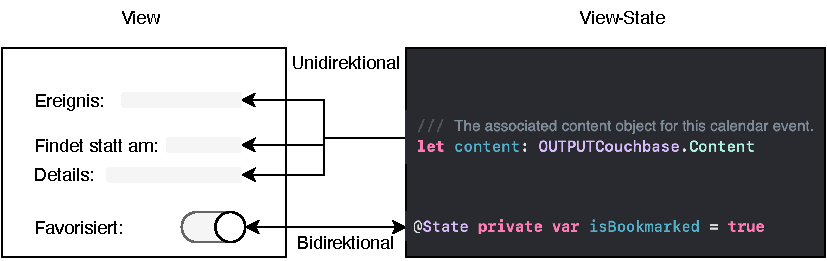
\includegraphics[width=\linewidth, bb=0 0 396 125]{swiftui.pdf}
\caption{Zwei wesentliche Arten des Datenflusses zwischen View und den in der View dargestellten Daten: unidirektional vs. bidirektional.}\label{fig:swiftui}
\end{figure}

\noindent \Cref{fig:swiftui} zeigt die zwei wesentlichsten Varianten, mithilfe derer Daten in der Ansicht dargestellt werden können: \textbf{unidirektional} und \textbf{bidirektional}. Bei der unidirektionalen Darstellung der Daten werden bei der Initialisierung der View die Daten im Konstruktor der View mitgegeben - da SwiftUI Views so genannte Structs sind, können die Daten im Verlauf der Zeit nicht mehr ändern (Struct-Felder sind \enquote{immutable}). SwiftUI rendert die assoziierten Elemente der View einmalig und verwendet diese nachfolgend zur Darstellung. Für viele Anwendungsfälle, in \Cref{fig:swiftui} anhang eines \enquote{Favorisieren-Buttons} illustriert, ist es jedoch notwendig, dass durch die View die dahinter liegenden Daten modifiziert werden. Hierfür wird der Property Wrapper \texttt{@State} bereitgestellt. Attribute, die hiermit ausgestattet werden, können während der Präsentation der View verändert werden. Eine Besonderheit hierbei ist, dass SwiftUI genau observiert, welche UI-Elemente durch das annotierte Attribut modifiziert oder konfiguriert werden, um bei einer Änderung des Attributs die entsprechenden Elemente neu zu rendern. Wird ein Datenattribut an eine Unteransicht weitergegeben, welche bspw. eine Detailansicht zu einem Objekt darstellt, dann wird das Attribut in der Unteransicht als \texttt{@Binding} referenziert.

\subsection{Coordinator-Pattern}

Um die Geschäftslogik der Anwendung von der Darstellungslogik weitestgehend zu separieren, kann das Coordinator-Pattern genutzt werden. Hierbei instanziiert die View ein eigenes Objekt, welches sie durch die \texttt{@StateObject} Annotation besitzt und kontrollieren kann, bspw. durch die Interaktion des Nutzers oder beim Erscheinen der Ansicht. Das Coordinator-Objekt macht die darzustellenden Datenattribute über die \texttt{@Published} Annotation nach außen verfügbar - so dass die View diese Datenattribute (ähnlich zu \texttt{@State} Datenattributen) verwenden und auf deren Änderungen reagieren kann.

\begin{figure}[H]
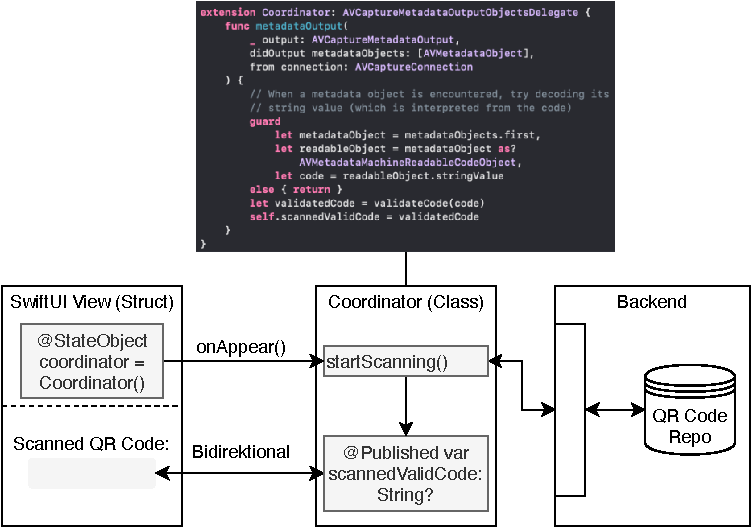
\includegraphics[width=\linewidth, bb=0 0 360 253]{coordinator.pdf}
\caption{Das Coordinator Pattern illustriert am Beispiel eines hypothetischen QR Code Scanners: Der Coordinator realisiert die Initialisierung des Scanners und die Validierung des Codes. Die View stellt den Code lediglich dar, sobald er gescannt wurde.}\label{fig:coordinator}
\end{figure}

\noindent In \Cref{fig:coordinator} ist das Pattern am Beispiel illustriert. Auch zu sehen ist hierbei, dass der Coordinator eine Klasse ist. Dies ist nützlich wenn bestimmte Protokolle (Swift-Interfaces) implementiert werden müssen, in diesem Beispiel \texttt{AVCaptureMetadataOutputObjectsDelegate} zur Reaktion auf gescannte QR Codes. In diesem Beispiel kann die View dieses Protokoll nicht implementieren, da das Protokoll implizit die Implementation durch eine Klasse erfordert.

\subsection{Environment-Pattern}

Als weiteres wichtiges Datenfluss-Pattern dient das Environment-Pattern. Hierbei wird, ähnlich zum Coordinator-Pattern, ein koordinierendes Umgebungsobjekt instanziiert und in der Besitz ergreifenden View als \texttt{@StateObject} markiert. Anschließend wird das Umgebungsobjekt im Environment der Unteransichten mitgegeben, über den ViewModifier \texttt{view.environmentObject()}. Dies ist zum Beispiel sinnvoll, wenn eine Unteransicht bestimmte Daten aus dem Kontext beziehen und/oder modifizieren möchte.

\begin{figure}[H]
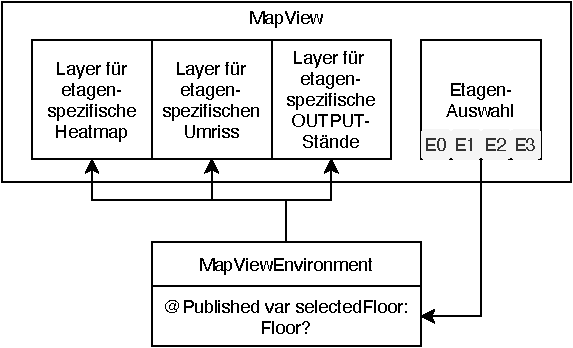
\includegraphics[width=0.75\linewidth, bb=0 0 275 167]{environment.pdf}
\caption{Das Environment Pattern illustriert am Beispiel der Map View: Die Map View erstellt ihr eigenes Environment und gibt dieses an ihre Unteransichten weiter. Somit kann die gewählte Etage von einer Unteransicht modifiziert werden, von anderen Unteransichten wird sie lediglich dargestellt.}\label{fig:environment}
\end{figure}

\noindent In \Cref{fig:environment} ist dieses Pattern am Beispiel illustriert. Ein großer Vorteil des Patterns ist, dass das über den ViewModifier weitergegebene Umgebungsobjekt transitiv an alle weiteren Unteransichten weitergeleitet wird, die sich möglicherweise in dieser Unteransicht befinden. Der Bezug des Objektes findet anschließend über \texttt{@EnvironmentObject var object} statt. Ein Problem hierbei ist, dass das Objekt nicht optional weitergegeben werden kann, was die Preview der SwiftUI Unteransichten erschwert. Die hierfür applizierte Lösung hierfür wird später im Konzeptkapitel näher beschrieben.

\subsection{View-Proxy-Pattern}

Die Grundlagen des Environment-Pattern und des Coordinator-Pattern können weiterhin genutzt werden, um bestimmte Bestandteile der Geschäftslogik im View-Proxy-Pattern zu separieren. Hierbei wird eine dedizierte View erstellt, deren Aufgabe es ist, bestimmte Datenverarbeitungsoperationen durchzuführen und bei Beendigung dessen die Produkte dieser Operation als Umgebungsobjekt bzw. Proxy-Objekt der inneren View bereitzustellen. Hierfür wird die innere View der Proxy View als \texttt{@ViewBuilder}-Closure übergeben. Ein klassisches Beispiel für das View-Proxy-Pattern ist der von SwiftUI standardmäßig bereitgestellte \texttt{GeometryReader}, welcher als View genutzt werden kann, um ein Proxy-Objekt für die Geometrie der View zu erstellen, bspw. um die Größe einer Ansicht zu bestimmen. Im Konzept der App wird dies später für die Initialisierung der Datenbank und Replikatoren adaptiert und an dieser Stelle noch einmal genauer beschrieben.

\subsection{Eventbasierte Datenflüsse}

Eventbasierte Datenflüsse stellen ein weiteres wichtiges Pattern für die Weitergabe von Daten dar. Bei den bisherigen Pattern wurden lediglich Methoden vorgestellt, mithilfe derer sich ein Datenfluss zwischen mehreren Views in \textit{derselben} View-Hierarchie realisieren lässt. In manchen Fällen ist es jedoch notwendig, dass bestimmte Datenverarbeitungsprozesse von der View-Hierarchie entkoppelt werden, beispielsweise bei periodischen Hintergrundprozessen. Um in diesem Fall dennoch bspw. eine entsprechende Meldung im UI anzuzeigen, können globale Events ausgelöst werden, die von Observern innerhalb der View aufgegriffen und zur Anzeige verarbeitet werden können. Hierbei kann das \texttt{NotificationCenter} genutzt werden, um Nachrichten auf einen Event-Bus zu pushen und innerhalb der View über einen so genannten \texttt{Publisher} zu empfangen. Auch dieses Pattern wird später noch an einem konkreten Beispiel im Rahmen des Implementationskonzeptes zu den Spiel-Errungenschaften gezeigt.

  \chapter{Analyse}\label{ch:analyse}

Bevor auf Grundlage der architekturellen Ideen aus \Cref{ch:grundlagen} ein konkretes Lösungskonzept entwickelt werden konnte, musste die bestehende App zunächst analysiert werden. Diese auf den Entwicklungsprozess vorbereitenden, analytischen Aspekte sollen in diesem Kapitel erörtert werden, um im nächsten Kapitel die konkreten Implementationskonzepte vorzustellen.

\section{Ermittlung einer Dialoglandkarte}

Zu Beginn der Analyse wurde die bestehende iOS App getestet, um alle möglichen Navigationswege und Dialoge zu sammeln und innerhalb einer Übersicht zu betrachten.

\begin{figure}[H]
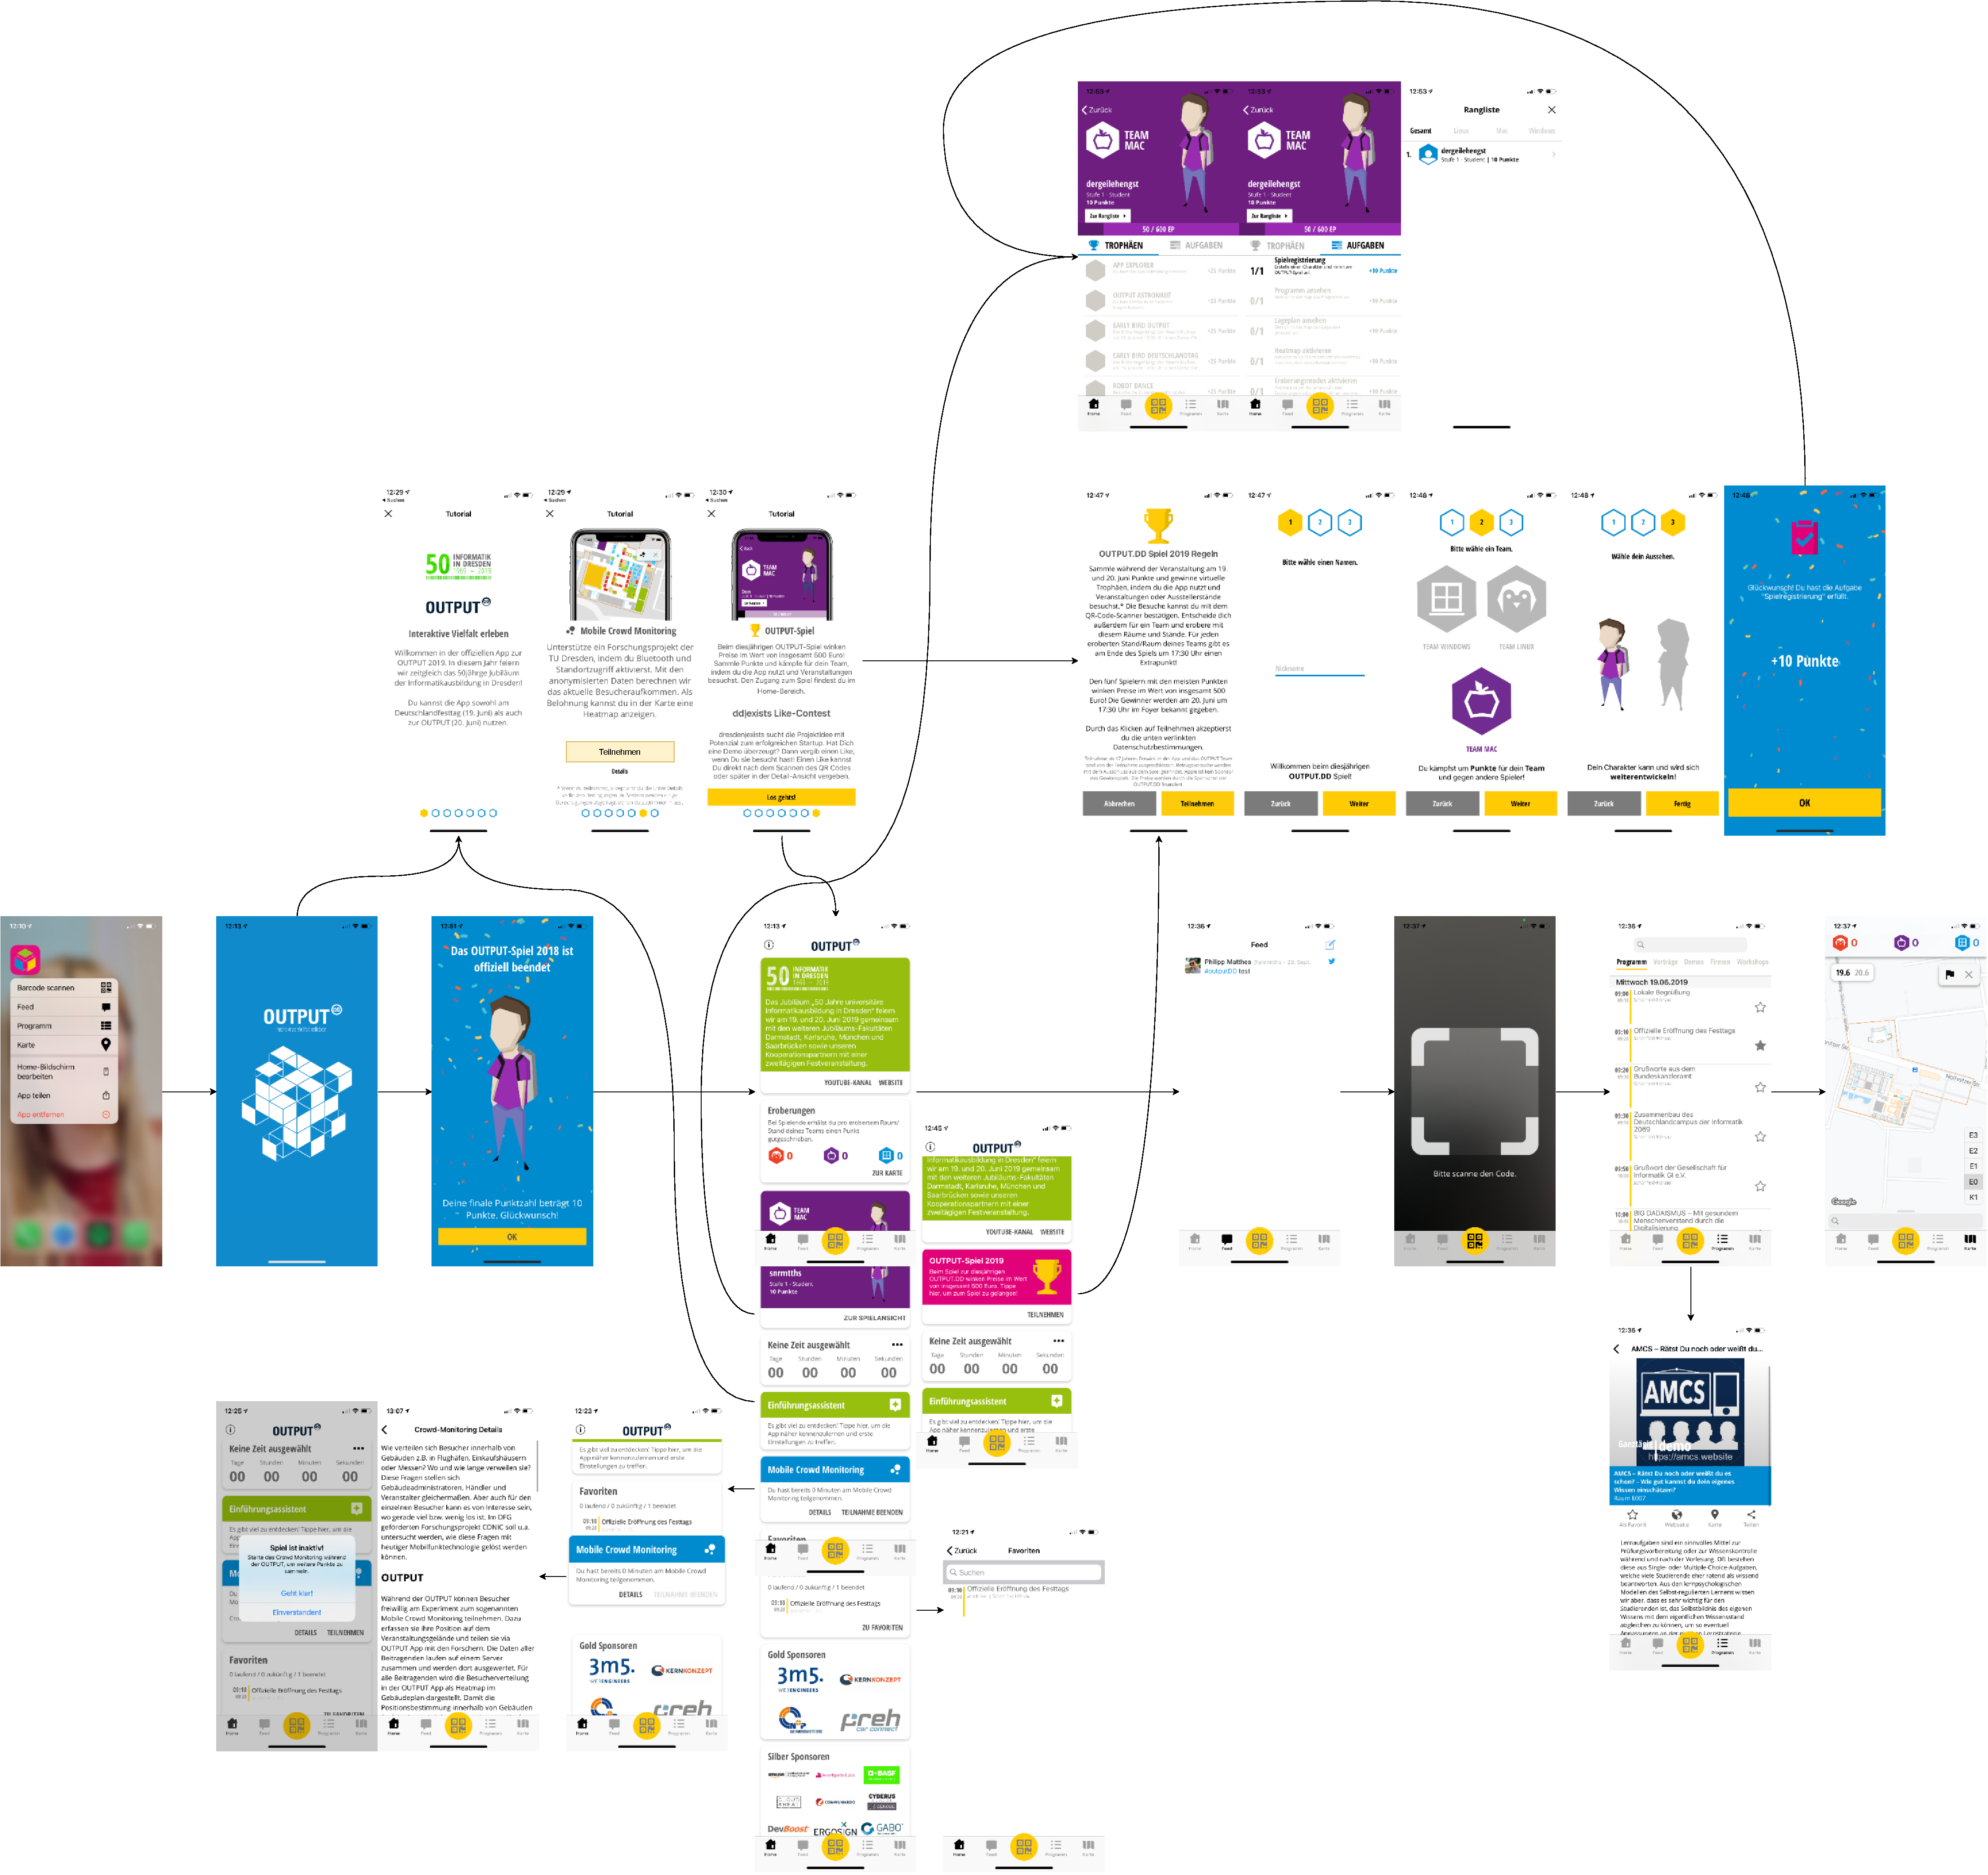
\includegraphics[width=\linewidth, bb=0 0 2123 2002]{mindmap.pdf}
\caption{Die erstellte Dialoglandkarte zur bestehenden Version der iOS App zeigt die Navigationswege innerhalb der App, sowie die genutzten UI-Elemente.}\label{fig:swiftui}
\end{figure}

Die in \Cref{fig:swiftui} gezeigte Dialoglandkarte suggeriert bereits die verschiedenen Gruppierungen von Ansichten, welche wir später zur Erstellung von neuen Packages heranziehen konnten. Zu sehen ist beispielsweise, dass die Spiel-Ansichten, der Einführungsassistent, oder bspw. auch die Kalender-Ansicht bereits gut voneinander separierbar sind. Die aufgezeichneten Navigationspfeile zwischen den Ansichten konnten genutzt werden, um die Datenflüsse hierbei vor der Erstellung des Konzeptes besser zu verstehen und die jeweils hierfür am Besten geeigneten Patterns zu finden.

\section{Struktur des Couchbase-Datenbank-Frameworks}




  \chapter{Konzept und Implementation}\label{ch:konzept}

Im Folgenden soll auf die in \Cref{ch:grundlagen} beschriebenen Patterns und Grundlagen zurückgegriffen werden und, zusammen mit den in \Cref{ch:analyse} analysierten Komponenten und Navigationswegen, das erstellte Konzept und die dazugehörige Implementation diskutiert werden.

\section{Konzeption einer Ordnerstruktur}

Die Konzeption einer Ordnerstruktur steht zu Beginn der Bearbeitung und Implementation der Applikation und soll für eine allgemeine Verbesserung der Applikationsstruktur gegenüber den in \Cref{ch:einleitung} genannten Strukturproblemen sorgen. Die Struktur ist dabei nach folgendem Regelwerk aufgebaut:

\begin{itemize}
\item Im Root-Verzeichnis des Repositories befinden sich Konfigurationsdateien des Package-Managers Cocoapods, Github-Workflows und weitere Hilfsdateien, die nicht direkt zur Codebasis der App gehören. Außerdem befindet sich an dieser Stelle das Applikationsverzeichnis.
\item In der obersten Applikationsebene befinden sich die komponentenspezifischen Ordner nach TLA, sowie die Applikationsklasse selbst und global konfigurierende Codefragmente und Artefakte (z.B. Lokalisierungsdateien, Info.plist).
\item Außerdem in der obersten Applikationsebene befindet sich ein Ordner \texttt{Resources}, in dem sich die Assets (z.B. AppIcon, UI-Elemente), jedoch auch Fonts, Lizenzen, eventuelle HTML-Templates oder andere Datenfragmente befinden.
\item Jede Komponente ist entweder separiert in weitere Teilkomponenten, oder besteht aus einer Auswahl aus den Unterordnern \texttt{Mocks}, \texttt{Views}, \texttt{ViewModels} oder anderen, Backend-Funktionalitäten kapselnden Ordnern.
\item Jedes \texttt{Mocks} Verzeichnis dient zur Bereitstellung von Mock-Objekten für die SwiftUI-Previews.
\item Jedes \texttt{ViewModels} Verzeichnis dient zur Bereitstellung von Modellen, die selbst nicht als Model Teil des Couchbase-Frameworks sind, sondern zusätzlich von Views zur Darstellung benötigt werden.
\item Jedes \texttt{Views} Verzeichnis beinhaltet die Ansichten der Komponente, die zur Darstellung der Applikation benötigt werden.
\end{itemize}

\noindent Die Applikation ist somit auf oberster Ebene vertikal geteilt, um eine bestmögliche funktionelle Separation der Module voneinander zu bestärken. Auf Komponenten-Ebene ist die Applikation horizontal geteilt, um die Ansichten bestmöglich von Datenmodellen und den dazugehörigen Backend-Funktionalitäten zu trennen. Außerdem soll darauf geachtet werden, dass die Klassen und Dateien innerhalb der jeweiligen Module möglichst als Präfix den Modulnamen tragen, beispielsweise \texttt{TwitterHTMLView} der Komponente Twitter, um sie später im Code besser voneinander unterscheiden und separieren zu können.

\section{Einführung eines Copyright-Templates}

Standardmäßig ergänzt XCode (iOS-IDE von Apple) beim Erstellen einer leeren Codedatei immer einen Copyright-Hinweis. Dieser ist jedoch nicht immer deskriptiv genug bzw. referenziert die dem Projekt beigefügte Lizenz nicht korrekt. Außerdem enthält der Copyright-Hinweis standardmäßig den gewählten Dateinamen, wodurch bei einer späteren Modifikation des Dateinamens auch immer gleichzeitig der Hinweis modifiziert werden muss, um Diskrepanzen zwischen dem Dateinamen und dem Hinweis zu verhindern. Deshalb wurde im Rahmen des Projektes ein Copyright-Template erstellt und in XCode, auf alle Entwickler des Projektes übergreifend, eingebunden.

\begin{figure}[H]
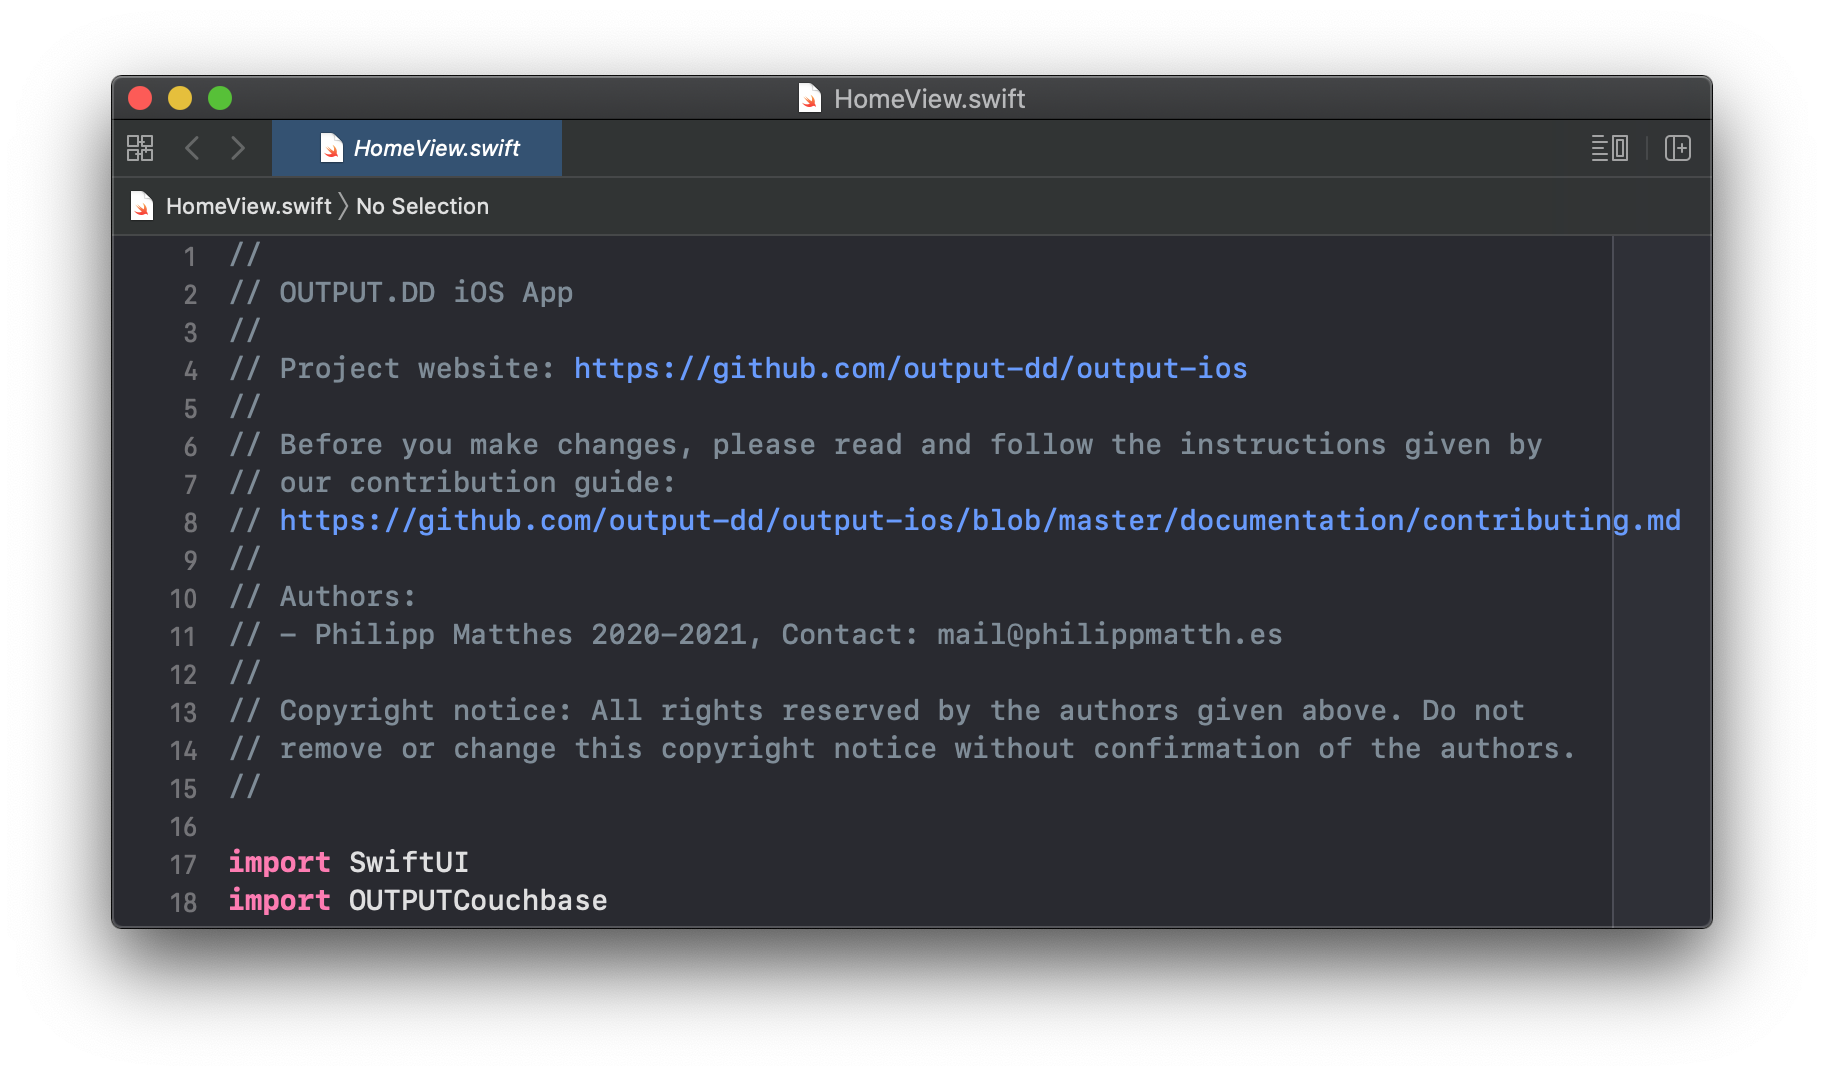
\includegraphics[width=\linewidth]{copyright.png}
\caption{Die erstellte Copyright-Template am Beispiel der HomeView.}\label{fig:copyright}
\end{figure}

\noindent Wie in \Cref{fig:copyright} sichtbar, enthält die Copyright-Template zusätzlich zu Hinweisen und Links über die Herkunft des Code-Fragmentes auch einen Link zu den Contribution-Guidelines, welche später im Konzept erläutert werden. Die Template ist bewusst so ausgelegt, dass sich mehrere Autoren inklusive ihrer Kontaktinformationen eintragen können. Letzteres ist wichtig, da sich im Projektteam noch nicht auf eine Lizenzierung der App unter einer Open-Source-Lizenz festgelegt wurde und daher die Codefragmente unter das Kopierrecht des Autors fallen. Sollte eine Weiterverwendung der Codefragmetes über den ursprünglich dafür bestimmten Rahmen stattfinden, so können die Autoren hierüber kontaktiert werden.

\section{Einführung von Codierungsrichtlinien}

Um das zusätzlich in der bestehenden Applikation identifizierte Problem mit der allgemeinen Degradation der Codequalität zu mitigieren und dieser präventiv entgegen zu wirken, wurde als statisches Codeanalysetool SwiftLint eingeführt und konfiguriert.

\begin{figure}[H]
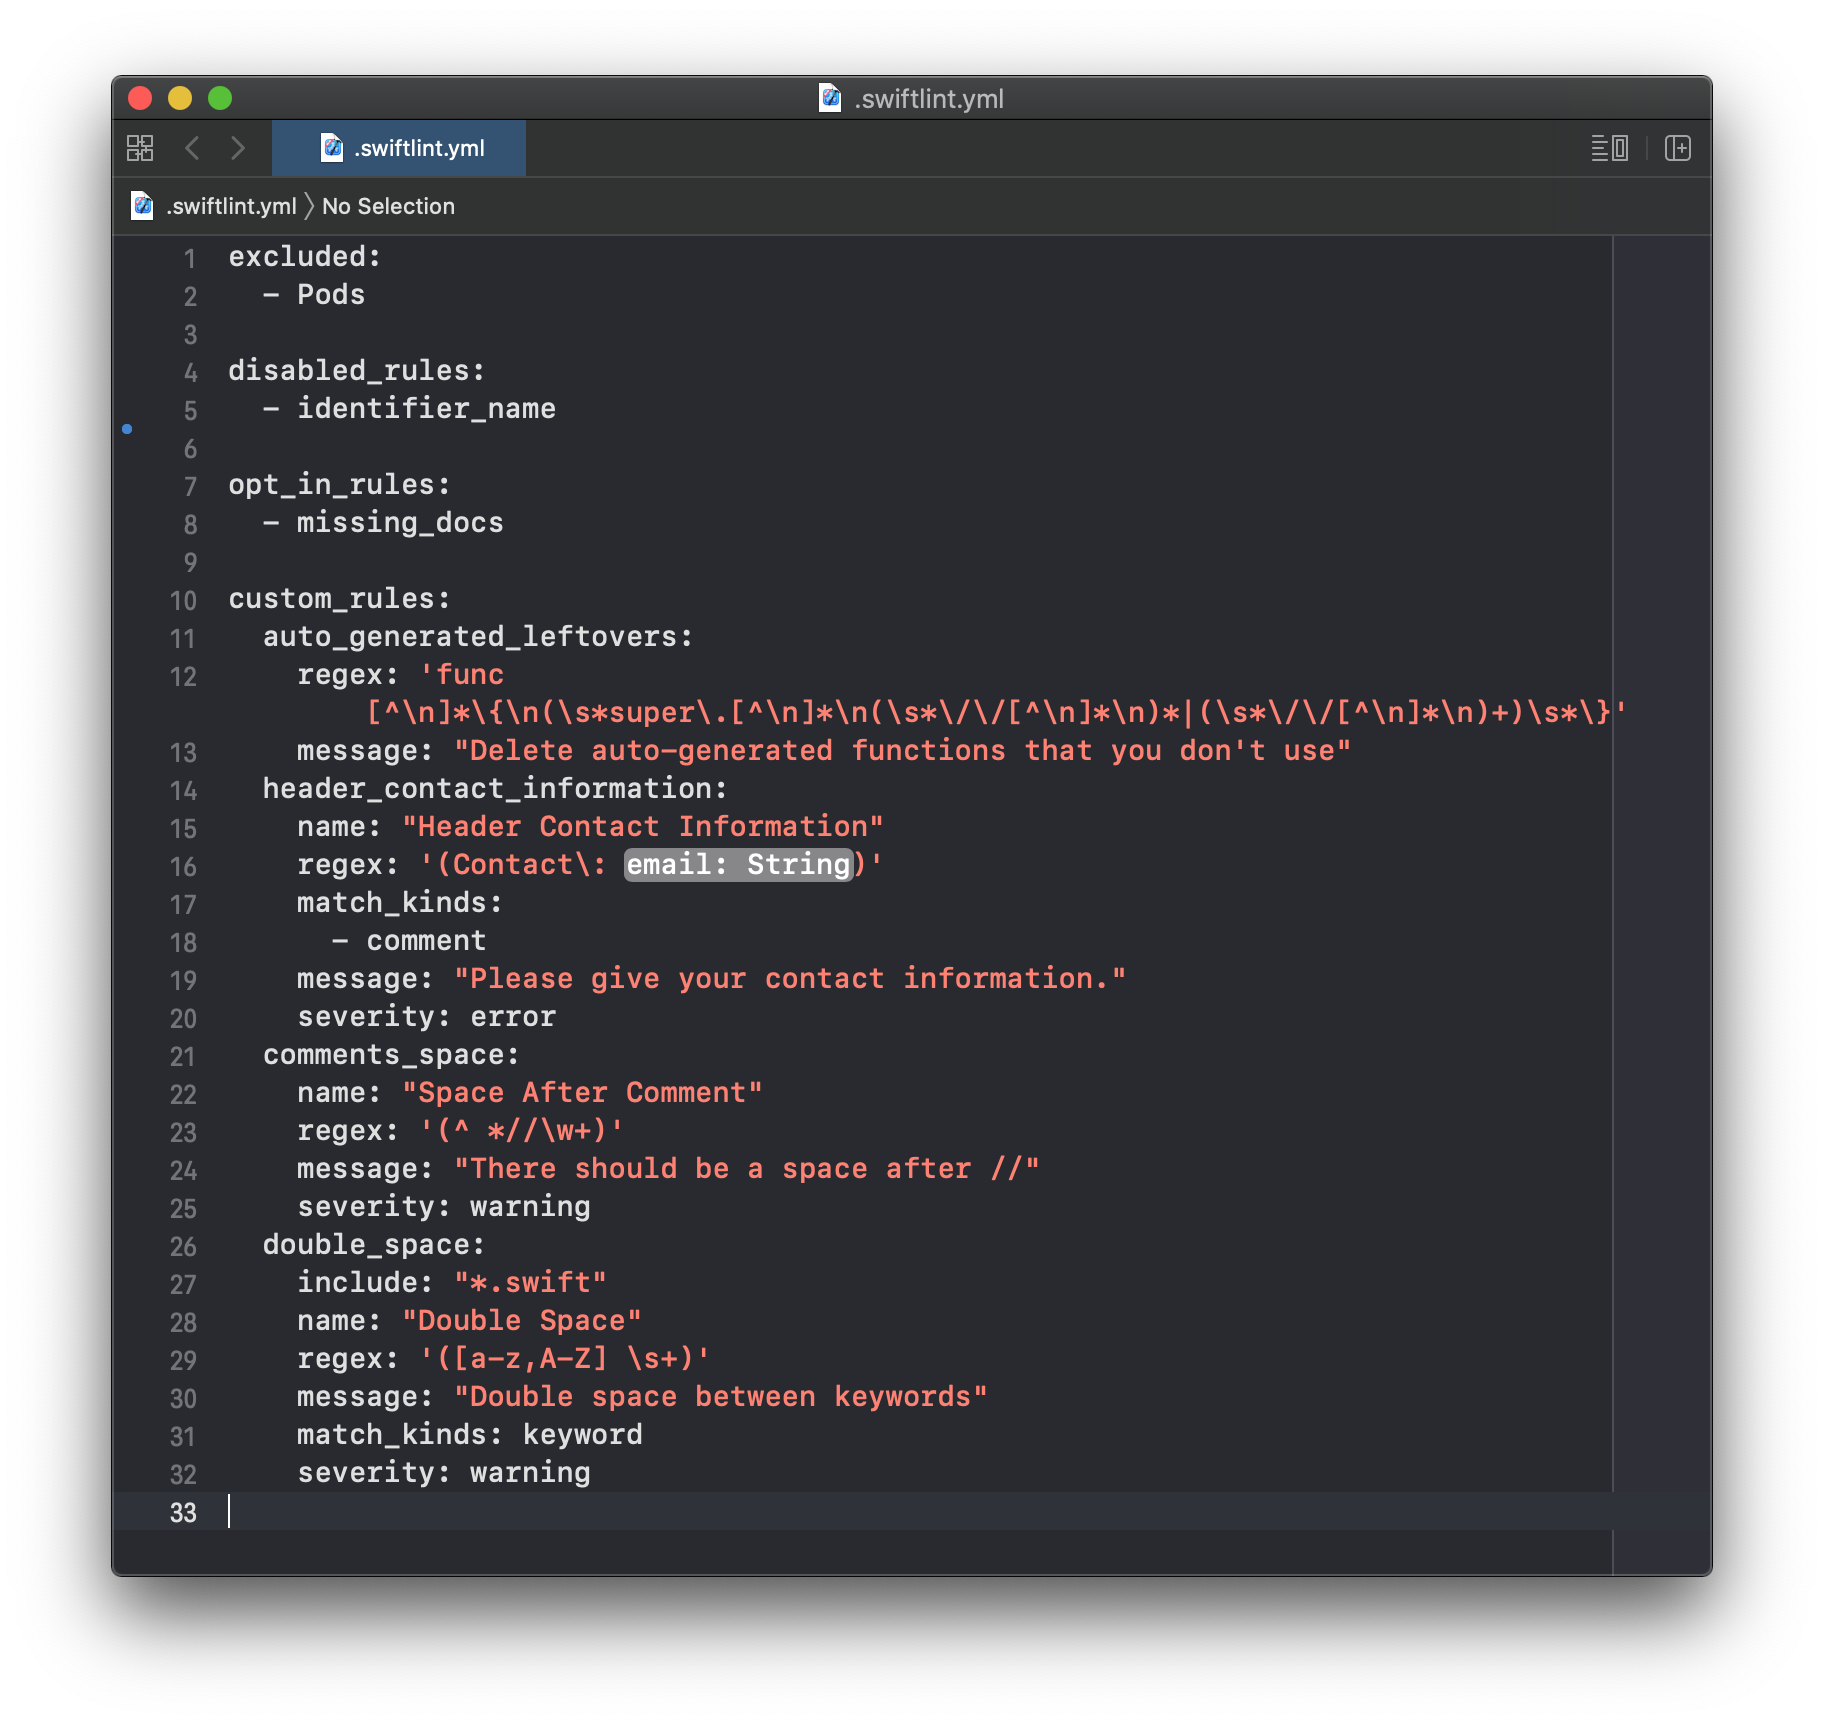
\includegraphics[width=\linewidth]{swiftlint.png}
\caption{Die Konfiguration des statischen Codeanalysetools SwiftLint.}\label{fig:swiftlint}
\end{figure}

\noindent In \Cref{fig:swiftlint} ist die Konfiguration von SwiftLint gezeigt. Neben gewöhnlichen Konfigurationen des Frameworks beinhaltet die Konfiguration auch eigene Regeln, darunter eine Regel, die auf das Vorhandensein des Copyright-Templates prüft. Das Tool wurde anschließend im Buildprozess von XCode integriert, so dass bei einer Verletzung der Codierungsrichtlinien diese innerhalb des Editors als Warnung (oder bei schwerwiegenden Verletzungen als Error) markiert wird und refaktorisiert werden kann.

\section{Implementation des Frontends}

Nach der Konzeption einer klaren Ordnerstruktur, sowie der Vorbereitung der Implementation mithilfe der Einführung des Copyright-Templates und der Installation eines statischen Code-Checkers wurde mit der Implementation des Frontends begonnen. Die Implementation fand hierbei entkoppelt vom Datenbank-Backend statt, indem für jede Ansicht temporäre ViewModels entworfen wurden, die zur Darstellung benutzt werden konnten. Dies ergab wesentliche Vorteile im Entwicklungsprozess:

\begin{itemize}
\item Die Ansichten konnten schnell mithilfe der SwiftUI-Preview erstellt werden, ohne eine aufwändige Anbindung des Datenbank-Backends oder eine entsprechende Daten-Initialisierung.
\item Die Ansichten konnten durch diesen Zwischenschritt leichter vom Datenbank-Backend separiert werden.
\end{itemize}

Außerdem konnte auf diese Weise in wenigen Wochen ein voll funktionsfähiges UI erstellt werden, lediglich mit einer fehlenden Anbindung an das Datenbank-Backend. Das UI konnte so bereits getestet und zwischen der iOS- und der Android-Version abgeglichen werden.

\begin{figure}[H]
\includegraphics[width=\linewidth, bb=0 0 2297 2000]{ui.pdf}
\caption{Die Hauptansichten des UI der neu implementierten App im Profil.}\label{fig:ui}
\end{figure}

\noindent In \Cref{fig:ui} werden die 5 Hauptansichten der App gezeigt, außerdem wurden noch einige weitere Ansichten (analog zur Dialoglandkarte) implementiert. Alle Ansichten orientieren sich hierbei am Aufbau der bisherigen Ansichten in der bestehenden App. Gleichzeitig wird das UI an vielen Stellen modernisiert, modularisiert und nutzerfreundlicher gestaltet. Zur Modernisierung gehört bspw. eine Implementation eines Dark-Mode Features, welches sich an der Systemeinstellung des Nutzers orientiert und bei Dunkelheit die Augen vor zu viel Helligkeit schützt. Außerdem wurden an verschiedenen Stellen bestimmte Animationen implementiert, bspw. bei dem Berühren eines Buttons, um die Benutzung der UI noch intuitiver und zufriedenstellender zu gestalten. Gleichzeitig wurde insbesondere auch auf Grundprinzipien des Usability Engineerings geachtet, sodass Buttons immer eine bestimmte Größe je nach Platzierung im UI besitzen und die meisten Interaktionen in der App in der unteren Hälfte des Bildschirms mit dem rechten Daumen getätigt werden können. Bei wichtigen Interaktionen erhält der Nutzer zudem ein haptisches Feedback. Zur Modularisierung des UI tragen bestimmte UI-Komponenten bei, die innerhalb verschiedener Ansichten mehrfach wiederverwendet werden können, wie eine (auch in \Cref{fig:ui} sichtbare) CardView oder ein eigener ViewPaginator. Nicht nur bei letzterem, sondern auch bei der Auswahl der Formen, Farben und Fonts wurde auf die Vorgaben aus der OUTPUD.DD Corporate Identity geachtet, so dass beispielsweise die Farbpalette übernommen wurde und ein wiederverwendbarer ViewModifier für die Applizierung des OpenSans-Fonts innerhalb von SwiftUI implementiert wurde. Außerdem wurde die Applikation vollständig internationalisiert, auf Grundlage der von SwiftUI bereitgestellten Funktion zur String Interpolation in Localizable.strings Dateien.

\paragraph{Reimplementation von weiteren Teilansichten: } Zusätzlich zu einer Reimplementation des gesamten UI, inklusive komplexerer Ansichten wie die Reward-Ansicht mit einer Konfetti-Animation, wurde in der Map-Ansicht das Google Maps Framework durch das MapBox Framework ersetzt. Vor dieser Entscheidung wurde anhand einer internen Team-Diskussion abgewägt, welches der beiden Frameworks zukünftig genutzt werden soll. Aufgrund der Nutzerfreundlichkeit, der leichten Anbindbarkeit und der Verwendung des Frameworks in anderen Projekten der Professur entschieden wir uns für MapBox. In der Twitter-Ansicht wurde während der Implementation des Frontends ein weiteres Problem identifiziert, welches darin bestand, dass das von der bestehenden App genutzte Twitter-Framework von Twitter nicht länger unterstützt wurde und damit die Gefahr bestand, dass in Zukunft diese UI-Komponente nicht mehr funktionieren könnte. Daher konzipierten wir als Lösung hierfür eine rein auf HTML basierende TwitterHTMLView, welche das von Twitter bereitgestellte Twitter Widget nutzt. Dies hat nicht nur den Vorteil, dass das nicht mehr unterstützte Framework entfernt werden konnte, sondern auch, dass kein API-Schlüssel mehr für die Verwendung notwendig ist.

\section{Integration einer CI-Pipeline}

Um die Applikation an verschiedene Tester über die von Apple bereitgestellte App \enquote{TestFlight} zu verteilen, bietet XCode die Möglichkeit, die Applikation zu signieren, in einem Archiv zu verpacken, dieses an die Plattform AppStore Connect zu übermitteln, und von dort (unter Vorausfüllung von Testinformationen) an die Tester zu übermitteln. Dieser Prozess ist jedoch sehr zeitaufwändig und dauert, je nach Tageszeit ca. 20-30 Minuten. Daher bat es sich an, die Applikation in einer Continuous-Integration-Pipeline einzubinden, welche diesen Prozess übernimmt. Hierzu wurde ein GitHub-Workflow adaptiert, der bereits für ein anderes iOS-Projekt (\enquote{Peerbridge} Blockchain Messenger) erstellt wurde. Der Workflow nutzt unter anderem das Framework Fastlane, um die Applikation zu archivieren und an die Tester vollautomatisch zu übermitteln. Hierfür sind einige technische Details von Relevanz, beispielsweise das Importieren des Signatur-Zertifikats in die CI-Pipeline, welche jedoch an dieser Stelle nicht weiter erläutert werden sollen. Für die Distribution wurden die technisch notwendigen Schritte in einem Delivery-Guide zusammengefasst, welcher im App-Repository unter \url{https://github.com/output-dd/output-ios/blob/master/documentation/delivery.md} (Zuletzt abgerufen am 31.1.2021) zu finden ist. Aus der Integration des Workflows bildet sich eine signifikante Zeitersparnis bei der Distribution der Applikation an die Tester. Die Applikation muss lediglich vom Entwickler mit einer Versionsnummer getaggt werden und die Bestimmungen von Apple erfüllen. Letztere sind konkret, dass die Build- und Versions-Nummer vor dem Taggen inkrementiert werden muss, sowie, dass die eventuell notwendigen Berechtigungen in der \texttt{Info.plist} Datei beschrieben sind.

\section{Fusion des Frontends mit dem Datenbank-Backend}

Auf Grundlage des implementierten Frontends und der CI-Pipeline konnten nun sukzessiv die einzelnen Komponenten und Ansichten um eine Backend-Persistierung erweitert und damit die übergangsweise genutzten ViewModels an geeigneten Stellen substituiert werden. Hierzu wurde das Datenbank-Backend über den Package-Manager Cocoapods als privates Pod hinzugefügt und die CI-Pipeline um die entsprechende Berechtigung ergänzt, damit diese auf das private Repository zugreifen kann. Anschließend wurden noch kleinere Änderungen am Datenbank-Backend, vor allem der Datenbank-Modelle vorgenommen, welche sich um Laufe der Zeit leicht geändert hatten. Mithilfe dieser Änderungen konnte nun auf Grundlage der in \Cref{ch:grundlagen} beschriebenen Patterns die Integration beginnen. \\

\subsection{Vorbemerkungen für die Darstellung der SwiftUI-Preview}

Wie in \Cref{ch:grundlagen} bereits angemerkt, ist ein zentrales Feature von SwiftUI die schnelle deklarative Erstellung von Ansichten. Dies wird unter anderem ermöglicht durch eine Echtzeit-Preview der Ansicht in XCode.

\begin{figure}[H]
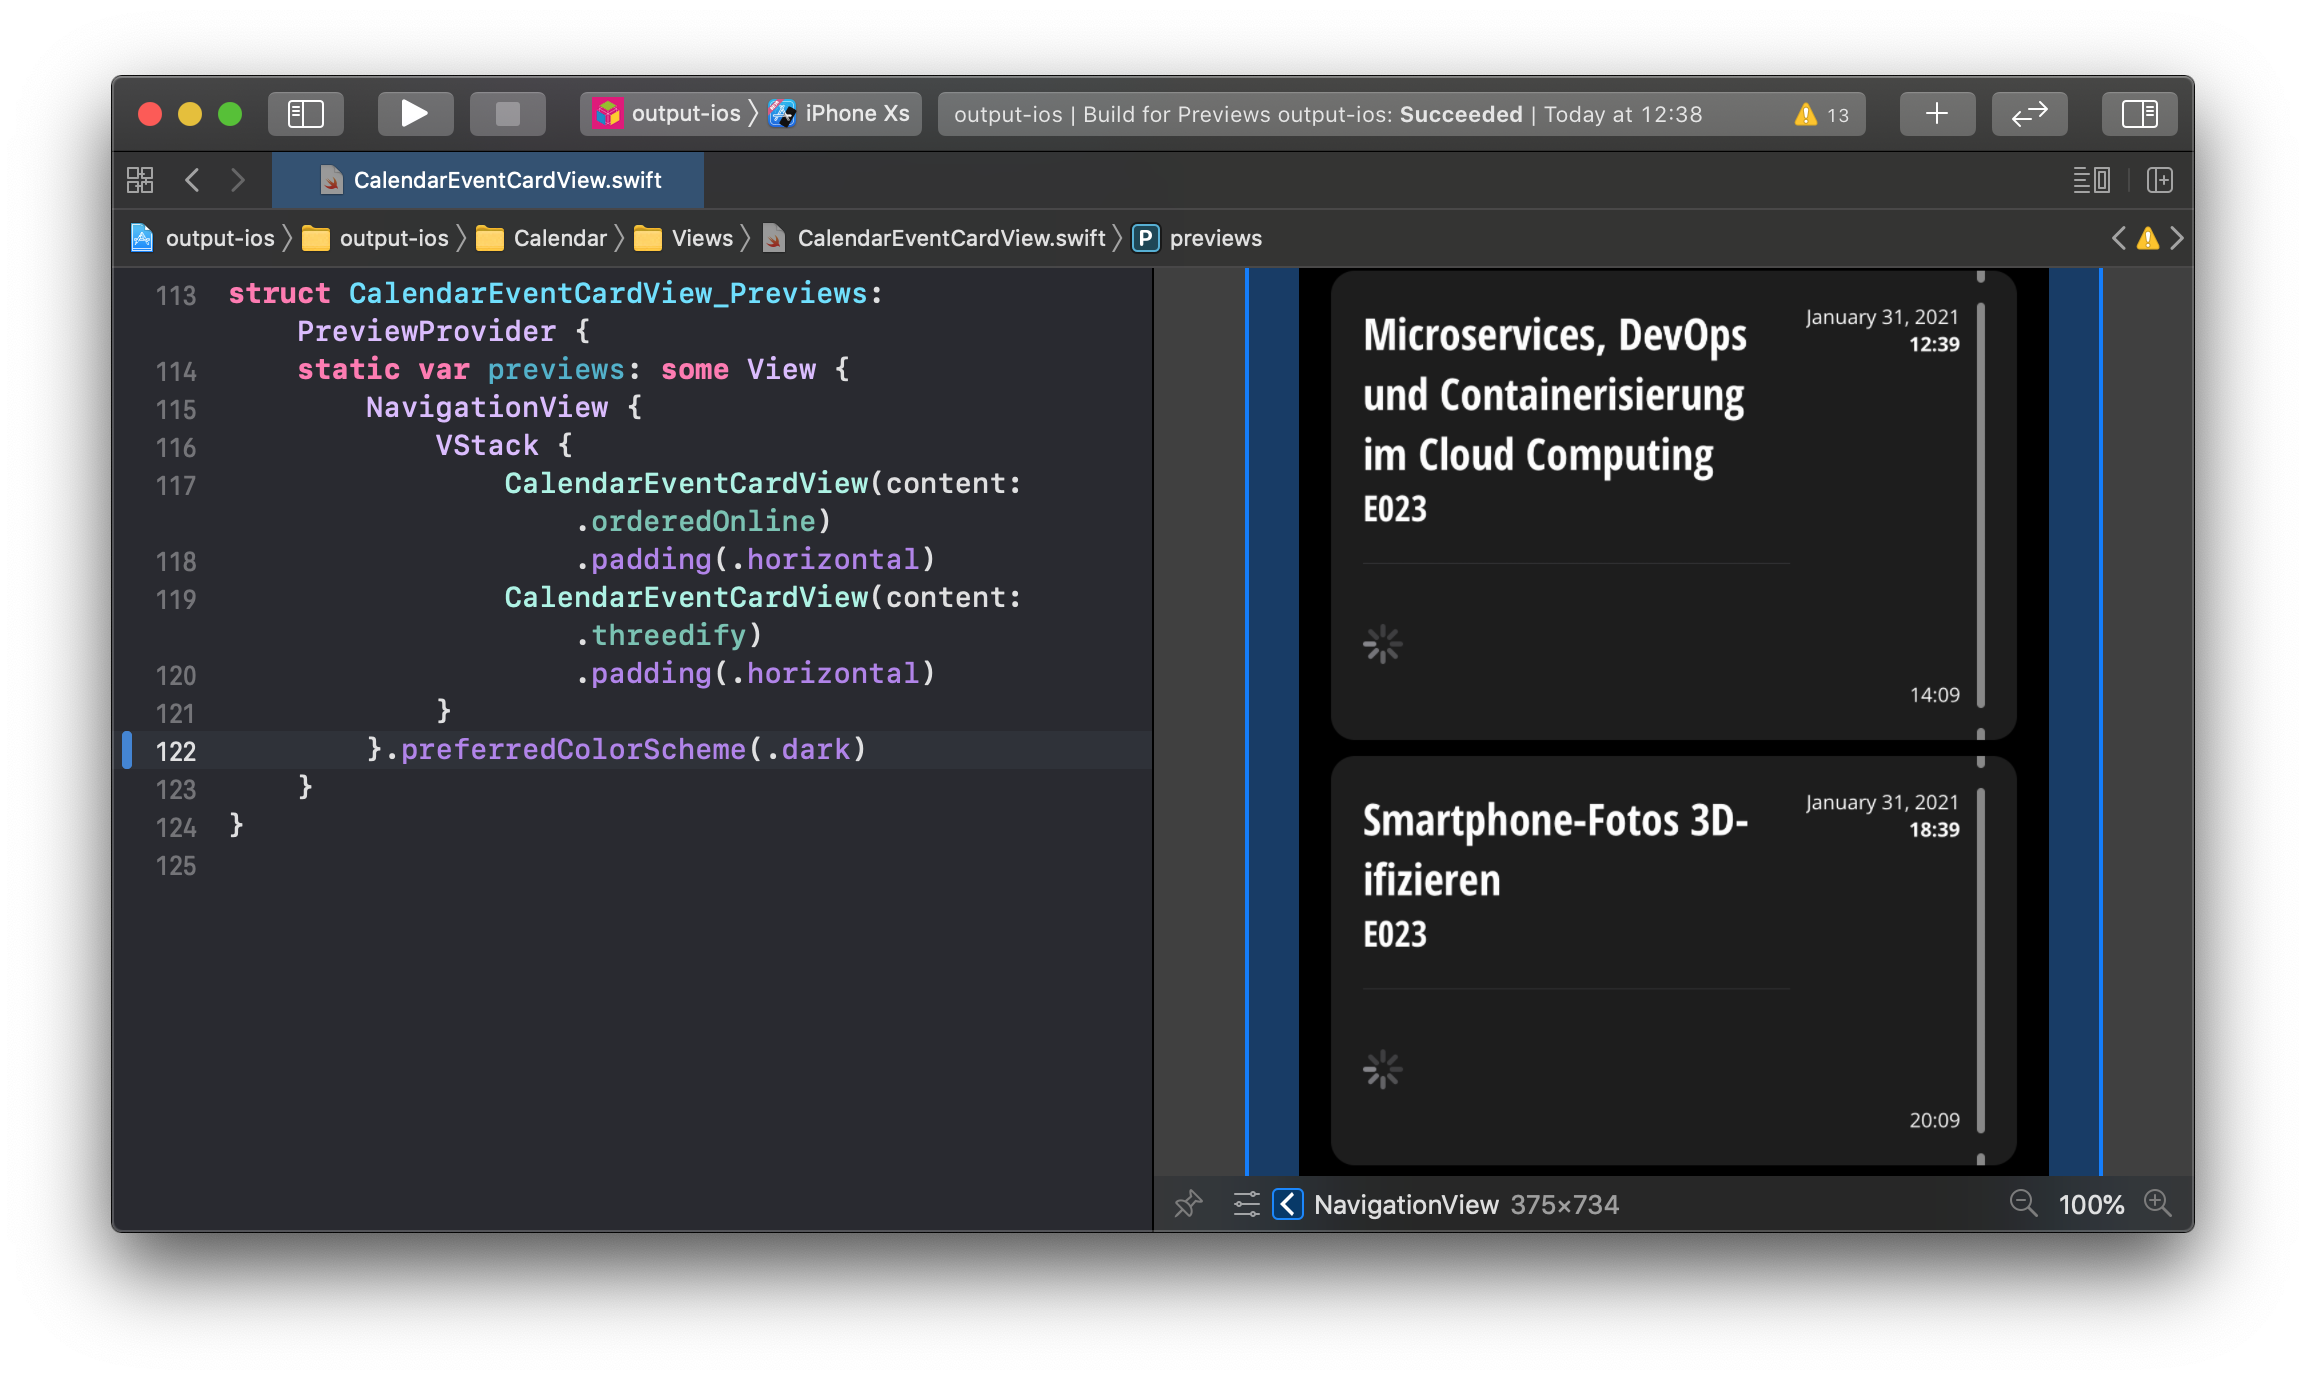
\includegraphics[width=\linewidth]{preview.png}
\caption{Die SwiftUI-Preview der \texttt{CalendarEventCardView} innerhalb von XCode.}\label{fig:preview}
\end{figure}

\noindent \Cref{fig:preview} zeigt eine solche Preview innerhalb XCode und wie diese konfiguriert werden kann. Hieraus entwickelt sich jedoch eine weitere Herausforderung bei der Integration des Datenbank-Backends in den Views, denn die Views sollten während der Preview nicht auf ein existierendes Datenbank-Backend angewiesen sein. Eine Vorinitialisierung des Datenbank-Backends in der Preview währe einerseits mit sehr viel zusätzlichem Boilerplate-Code verbunden, andererseits könnte die Preview dann nicht schnell editiert werden, weil bei jeder Änderung der Ansicht das Datenbank-Backend wieder initialisiert werden müsste. Im Folgenden Abschnitt wird die hierfür konzipierte Lösung gezeigt.

\subsection{Nutzung des Environment- und Coordinator-Patterns für die Anbindung der Views}

Um in der Preview der Views auf die zuvor erstellten Mocks zur schnellen Darstellung und Änderung der Ansicht zugreifen zu können und gleichzeitig beim Testen der Applikation auf dem Simulator oder dem physischen Gerät die initialisierte Datenbank zu nutzen, werden die anzubindenden Views mit jeweils einem \texttt{DemoCoordinator} oder einem \texttt{PersistedCoordinator} ausgestattet. Die jeweiligen Koordinatoren erben hierbei von der selben Klasse \texttt{Coordinator} - welche die benötigten Schnittstellen zur Verfügung stellt. Die zwei unterschiedlichen Subklassen-Koordinatoren unterscheiden sich infolge dessen nur darin, ob zum Prozessieren bzw. Holen der Daten die Datenbank genutzt wird, oder lediglich Mock-Objekte für die Preview zurückgegeben werden.

\begin{figure}[H]
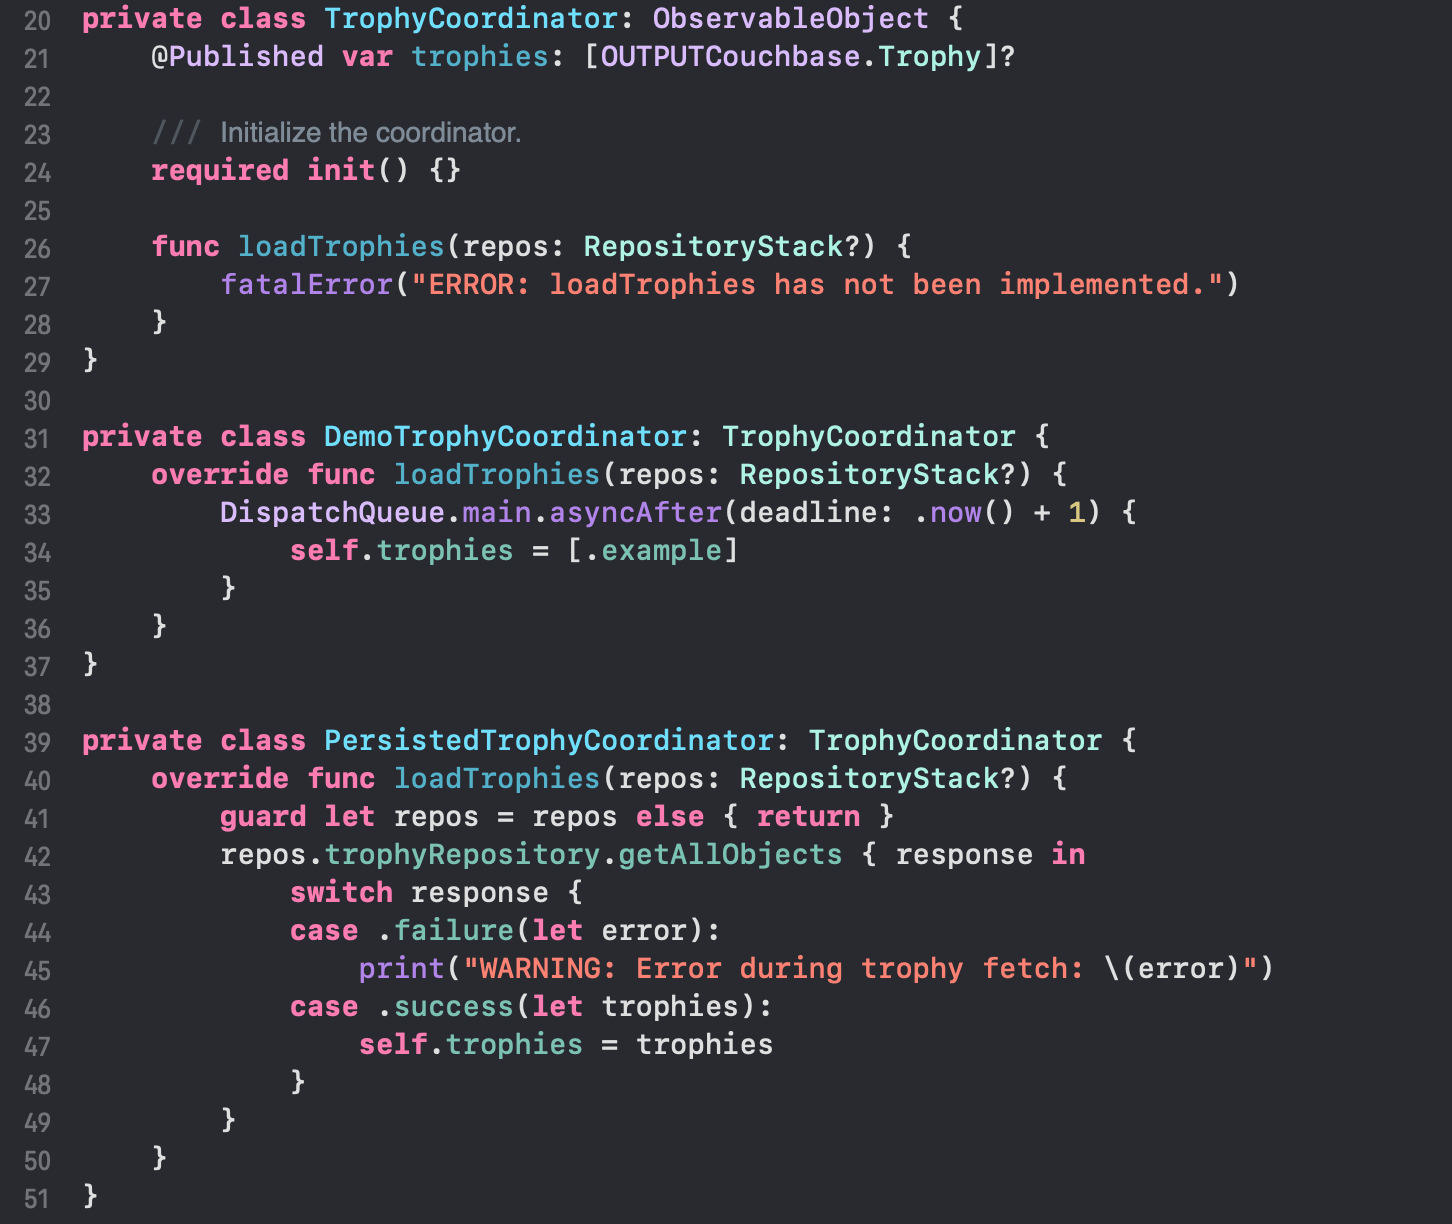
\includegraphics[width=\linewidth]{demo-persisted.png}
\caption{Das Coordinator-Pattern angewandt am Beispiel der Spiel-Trophäen, um eine schnelle SwiftUI-Preview ohne Daten-Initialisierung zu gewährleisten.}\label{fig:demo-persisted}
\end{figure}

\noindent Zur Illustration ist dieses Pattern beispielhaft in \Cref{fig:demo-persisted} an der Implementation gezeigt. Der \texttt{TrophyCoordinator} gibt die Schnittstellen vor, an dieser Stelle die geladenen Trophäen (bidirektional referenzierbar durch die Ansicht) sowie eine Funktion zum Laden der Trophäen. Der \texttt{DemoTrophyCoordinator} lädt lediglich gemockte Beispiel-Trophäen nach einer kurzen Verzögerung, um den Ladeprozess zu simulieren. Der \texttt{PersistedTrophyCoordinator} greift auf die Repositories und damit auf die Datenbank zu, um die tatsächlich persistierten Trophäen zu laden.

\begin{figure}[H]
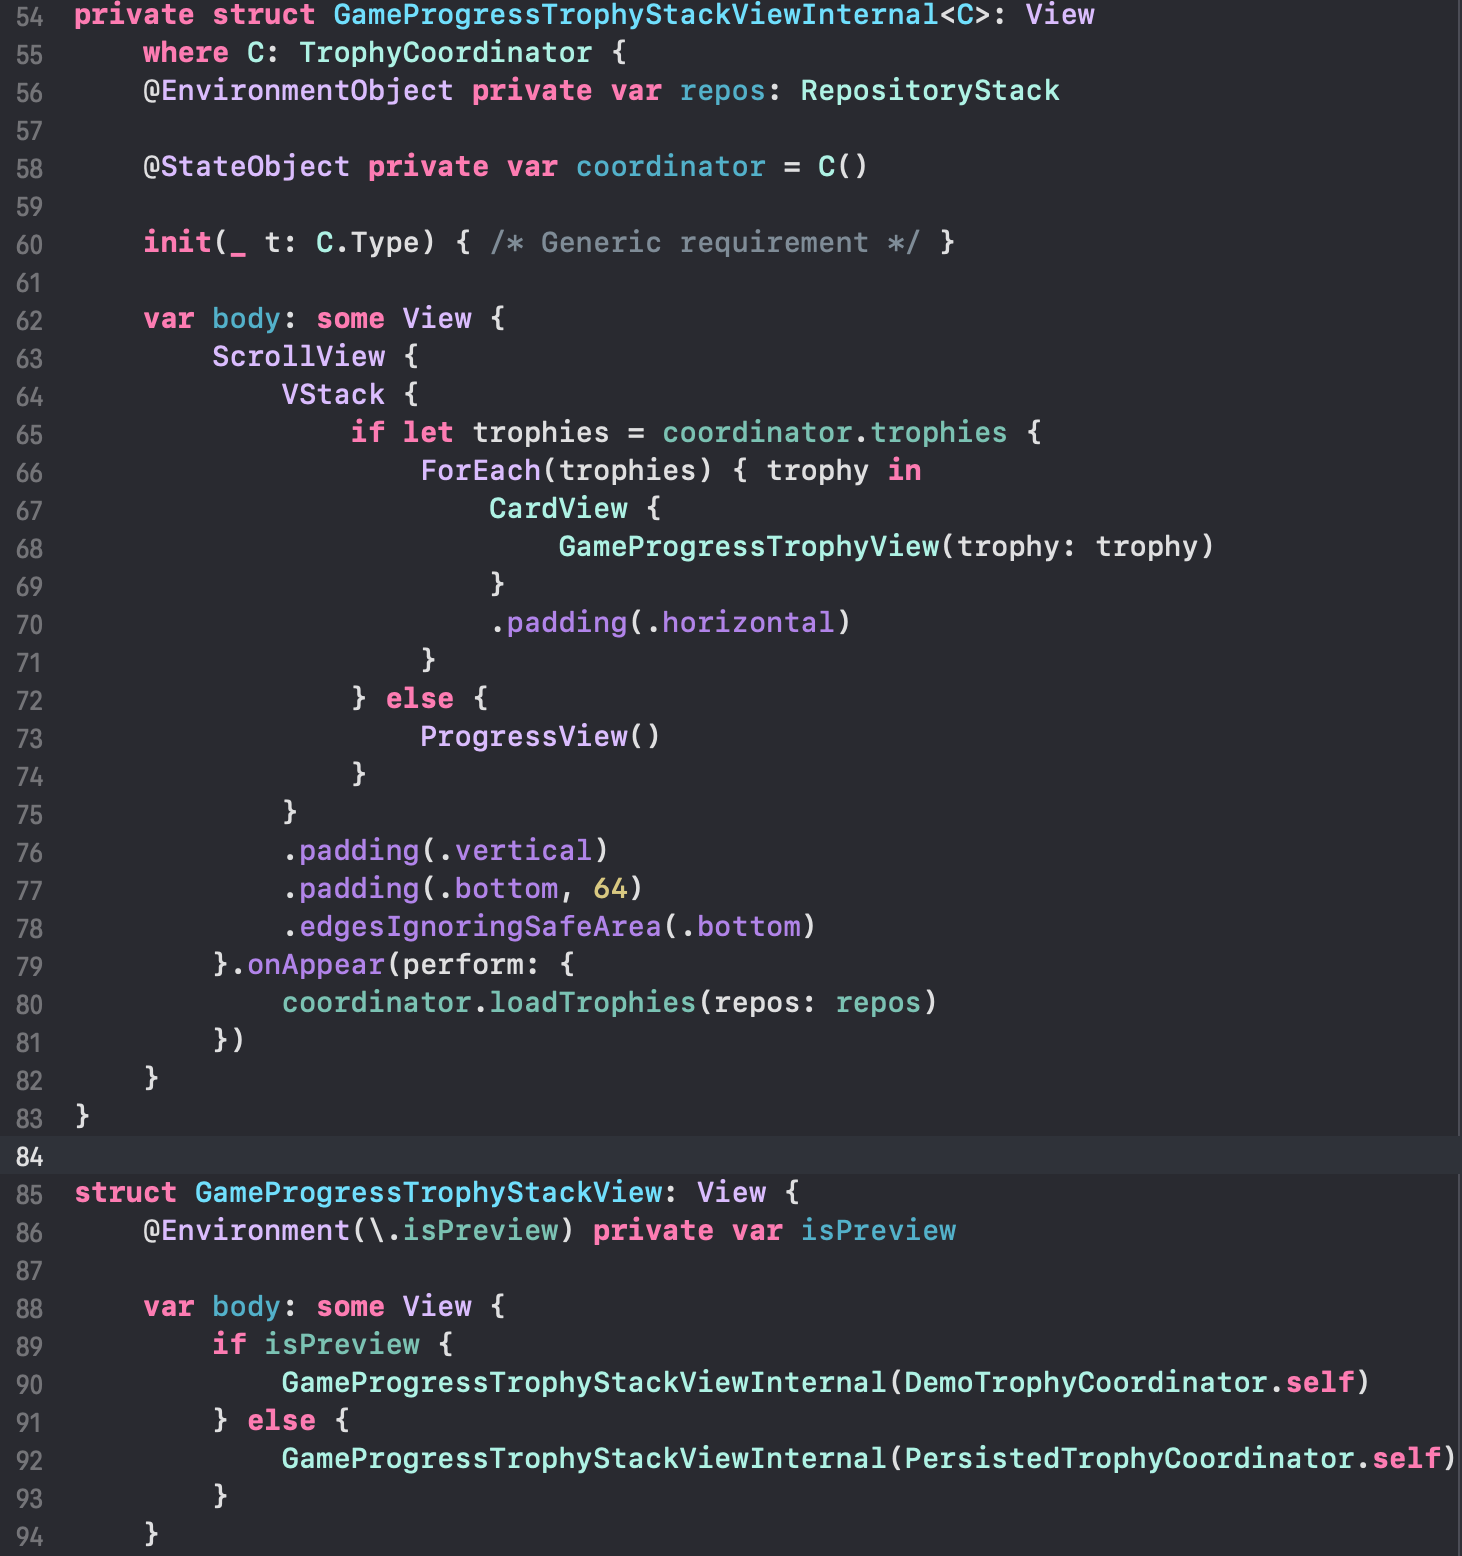
\includegraphics[width=\linewidth]{demo-persisted-view.png}
\caption{Die Anbindung der Koordinatoren an die View im Beispiel der \texttt{GameProgressTrophyStackView}.}\label{fig:demo-persisted-view}
\end{figure}

\noindent Die Integration der Koordinatoren erfolgt über die Übergabe als generischen Typparameter im Konstruktor der View. Um die Koordinatoren außerhalb der View-Code-Datei unsichtbar zu machen und nicht den globalen Scope zu verschmutzen, in dem die Koordinatoren keine Bedeutung haben (da sie sich nur auf die einzelne View beziehen) wird die Entscheidung, welcher Koordinator genutzt wird, durch ein Umgebungsattribut \texttt{isPreview} inferiert. Dieses Umgebungsattribut wird aus der Prozessumgebung bezogen, welche Informationen beinhaltet, ob es sich bei der aktuellen Ausführung um eine SwiftUI-Preview-Umgebung handelt, oder nicht. Entsprechend wird der \texttt{DemoCoordinator} nur genutzt, wenn es sich um eine SwiftUI-Preview-Umgebung handelt. Dieses Pattern wurde auf alle Views angewandt, welche bei der Ausführung auf dem Gerät (physisch oder Simulator) mit der Datenbank kommunizieren.

\subsection{Nutzung des Proxy-Patterns für die Initialisierung der Datenbank}

Um die Datenbank zu initialisieren, wird auf das in \Cref{ch:grundlagen} erläuterte Proxy-Pattern zurückgegriffen.

\begin{figure}[H]
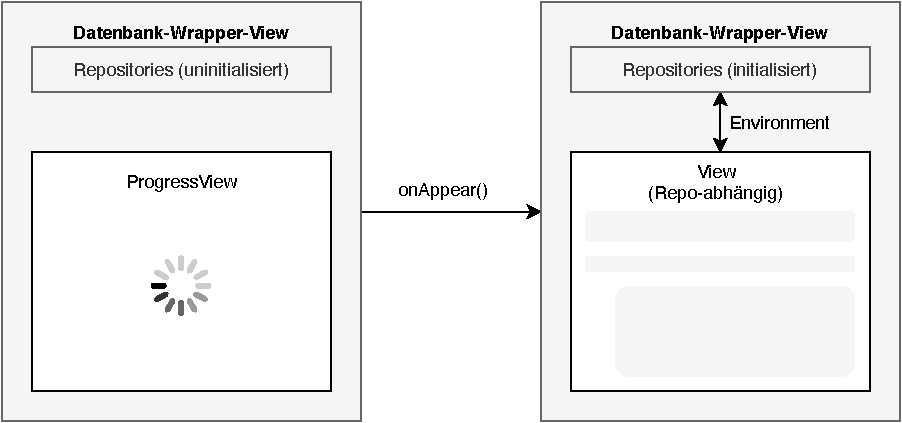
\includegraphics[width=\linewidth, bb=0 0 432 203]{proxy.pdf}
\caption{Abstrakte Übersicht über die Initialisierung der Datenbank.}\label{fig:proxy}
\end{figure}

\noindent \Cref{fig:proxy} zeigt die Initialisierung der Datenbank. Hierzu werden die datenbankabhängigen Ansichten als innere View mitgegeben. Sobald nun die Gesamtansicht erscheint (in diesem Fall beim Start der App) wird zunächst ein Loading-Indicator angezeigt und die Datenbank initial erstellt bzw. geladen.  Anschließend werden die Repositories auf der Datenbank initialisiert und über das Environment der Ansicht an die Unteransichten übergeben. Die Unteransichten besitzen hierdurch die Möglichkeit, über die Umgebung auf die Repositories und somit auch auf die persistierten Objekte zuzugreifen. Gleichzeitig wird die Datenbank auch wieder deinitialisiert, sobald die Applikation geschlossen wird. Dies ist in SwiftUI sehr einfach möglich über die Nutzung von \texttt{onAppear()} und \texttt{onDisappear()}. Es handelt sich infolgedessen insgesamt um einen eher SwiftUI-orientierten Lösungsansatz. Alternativ könnte als nicht direkt an SwiftUI gekoppelte Lösung auch bspw. ein Singleton-Pattern genutzt werden, indem die Datenbankrepositories auf einem Singleton statisch initiiert und verfügbar sind. Hierbei könnte das Singleton jedoch auch innerhalb der Proxy-View initialisiert werden, oder unabhängig von SwiftUI innerhalb der Methoden eines \texttt{AppDelegate}. Beide Varianten, also einerseits die Nutzung des Environment zusammen mit einer Proxy-View und andererseits die Nutzung eines Singletons, wurden getestet und gegeneinander im Rahmen der Entwicklung abgewägt. Wegen der allgemeinen SwiftUI-Orientierung der Neuimplementation wurde sich in der iOS-Implementierung für ersteres entschieden.

\subsection{Testen der Datenbankfunktionalität}

Um die Anbindung der Datenbank zu testen, wurden im Rahmen der Implementation zu Testzwecken auch mehrere Daten-Initialisierer implementiert. Hierbei wurden in die Repositories beim erstmaligen Start der Applikation teils vorliegende und teils zufällig generierte Objekte geschrieben, um die Darstellung der jeweiligen Daten innerhalb der angebundenen UI-Komponenten zu testen. Unter anderem wurden hierzu auch Test-Skripte entwickelt, bspw. um die Heatmap auf Grundlage der vorliegenden GeoJSON-Umrisse der Etagen des Andreas-Pfitzmann-Baus zu generieren. Somit konnte für die angebundenen Ansichten sichergestellt werden, dass unter Existenz von Objekten in der Datenbank diese korrekt behandelt und dargestellt werden. Gleichzeitig konnte auch die Performanz der Applikation getestet werden, beispielsweise durch die Generierung von mehreren tausenden Einträgen im Leaderboard der Gamification.

\subsection{Anbindung der Synchronisationskomponente}

Ähnlich zur Integration der Datenbank konnte für die Anbindung der Synchronisationskomponente auch das View-Proxy-Pattern genutzt werden. Hierbei wird zusätzlich zur Couchbase-Datenbank, die (neben ihrer Schnittstellen) lediglich eine Referenz zu einer physisch auf dem Dateisystem vorliegenden Datei darstellt, zwei verschiedene Replikatoren für unterschiedliche Repositories implementiert. Aus Datenschutz- und Datensicherheitsgründen wurden die Repositories des Couchbase-Datenbank-Frameworks in \texttt{personal} und \texttt{shared} separiert, wobei ersteres nur individuell für den Nutzer selbst verfügbar ist und letzteres für alle Nutzer. Die \texttt{shared} Repositories beinhalten öffentlich verfügbare Daten, wie bspw. die Sponsoren und Kalenderereignisse. Innerhalb der \texttt{personal} Repositories befinden sich vorrangig Daten zum individuellen OUTPUT.DD-Spieler und zur Favorisierung von Ereignissen. Entsprechend benötigt der Replikator für die \texttt{personal} Repositories eine zufällig generierte Authentifikation, welche zum jeweiligen Spieler des OUTPUT.DD-Spiels gehört, bei einem zum Server-Backend gehörenden Registrierungsservice erstellt und in den \texttt{UserDefaults} der Applikation persistiert wird. Somit wird der \texttt{personal} Replikator erst verbunden, wenn der Nutzer einen Spieler im OUTPUT.DD-Spiel (und damit seine Authentifikation) registriert hat. Gleichzeitig bleibt der \texttt{shared} Replikator stets auch ohne Authentifikation aktiv, um die öffentlichen Daten mit dem Server-Backend zu synchronisieren. Diese Funktionalität wurde innerhalb eines \texttt{CouchbaseManagers} implementiert, welcher durch eine eigene Proxy-View initialisiert wird. Lediglich für die Registrierung des Spiels wird der \texttt{CouchbaseManager} an die Unteransichten weitergegeben, damit an dieser Stelle, bei erfolgreicher Registrierung und Authentifikation, der \texttt{personal} Replikator gestartet werden kann und unverzüglich alle Daten der \texttt{personal} Repositories synchronisiert werden.

\subsection{Testen der Synchronisation}

Zum Testen der Replikatoren wurde ein im Rahmen der Implementation des Couchbase-Datenbank-Frameworks enstandenes Docker-Test-Setup genutzt. In diesem Test-Setup sind alle notwendigen Services enthalten, welche für die Realisation der Synchronisation notwendig sind. Darunter:

\begin{itemize}
\item Der Couchbase Server, in welchem eine zentrale Referenz der Datenbank gespeichert wird.
\item Das Couchbase Sync Gateway, welches eine Synchronisationsschnittstelle für die Replikatoren bereitstellt.
\item Der Registrierungsservice, welcher zur Registrierung eines neuen Spielers genutzt wird.
\item Der Sync Service, welcher die Couchbase-Daten mit der OUTPUT.DD-Website synchronisiert und bestimmte Daten aggregiert.
\item Der Couchbase Update Notifier, welcher den Sync Service von bestimmten Aktualisierungen in der Datenbank notifiziert.
\end{itemize}

\noindent Dieses Test-Setup kann mithilfe von Docker-Compose lokal auf dem Entwicklersystem gestartet werden und als Endpunkt für die Replikatoren und die Spielerregistrierung referenziert werden. Mithilfe des Docker-Test-Setups konnte die Replikator-Funktionalität erfolreich sichergestellt werden. Außerdem konnten einige Probleme in der Implementation des Test-Setups identifiziert werden. Darunter ein Problem bei der Registrierung eines neuen Spielers, bei dem der Registrierungsservice mit einem internen Server-Error (Code \texttt{500}) antwortet, wenn der Spielername bereits vergeben ist, sowie eine fehlerhafte Aggregierung des Player-Modells im \texttt{shared} Repository, welches dazu führt, dass kein Leaderboard dargestellt werden konnte. Die Probleme wurden im Projektteam besprochen und die entsprechenden Fixes beim zuständigen Entwickler eingeleitet.

\section{Listener- und Eventbasierte Anbindung der Gamification}

Nachdem das Frontend der Applikation, sowie die Datenbank und die Synchronisationsfunktionalität implementiert werden konnte, wurden anschließend die in der Gamification der App erreichbaren Trophäen und Aufgaben analysiert und eine Implementation der jeweils dahinter stehenden Logik geplant. Hierzu wurde zunächst eine Übersicht über die vorhandenen Trophäen und Tasks erstellt und anhand dessen die Kriterien für die Freischaltung festgelegt, damit diese Kriterien möglichst einheitlich zwischen der iOS- und Android-Version der App gehandhabt werden. Außerdem wurden die Trophäen und Aufgaben in jeweils zwei Untergruppen separiert:

\begin{itemize}
    \item \textbf{Datenbasierte} Errungenschaften, welche durch die Änderung oder Erstellung von bestimmten Objekten in der Datenbank erreicht werden können. Beispiele hierfür sind das Speichern eines gescannten QR Codes oder die Registrierung eines neuen Spielers.
    \item \textbf{Interaktionsbasierte} Errungenschaften, die durch eine bestimmte Interaktion mit Elementen der App erreicht werden können, welche jedoch nicht direkt eine Änderung der innerhalb der Datenbank persistierten Daten zur Folge hat. Ein Beispiel hierfür ist der Aufruf einer bestimmten Ansicht.
\end{itemize}

\noindent Die Freischaltung bestimmter Errungenschaften kann hierbei als Hintergrundprozess gesehen werden - der Nutzer führt bestimmte Aktionen aus, welche observiert werden und bei Zutreffen des jeweiligen Kriteriums der Errungenschaft eine Freischaltung zur Folge hat. Die observierenden Komponenten der Applikation entscheiden also selbstständig bei der Benachrichtigung durch das jeweilige Ereignis (datenbasiert oder interaktionsbasiert), ob die jeweilige Trophäe oder die Aufgabe freigeschaltet werden soll. Nach diesem Paradigma konnten die Errungenschaften gut von der sonstigen Darstellungs- und Geschäftslogik der App separiert werden.

\subsubsection{Implementation der datenbasierten Errungenschaften}

Da sich die Freischaltung von datenbasierte Errungenschaften direkt von der Änderung bestimmter Datenmodelle innerhalb der Datenbank ableitet, wurden für die Implementation Datenbank-Listener für die jeweiligen Datenmodelle genutzt, welche durch das Couchbase-Repository-Framework bereitgestellt wurden. Hierbei durchläuft jeder Observer nach der Initiation der Repositories folgenden Algorithmus:

\begin{figure}[H]
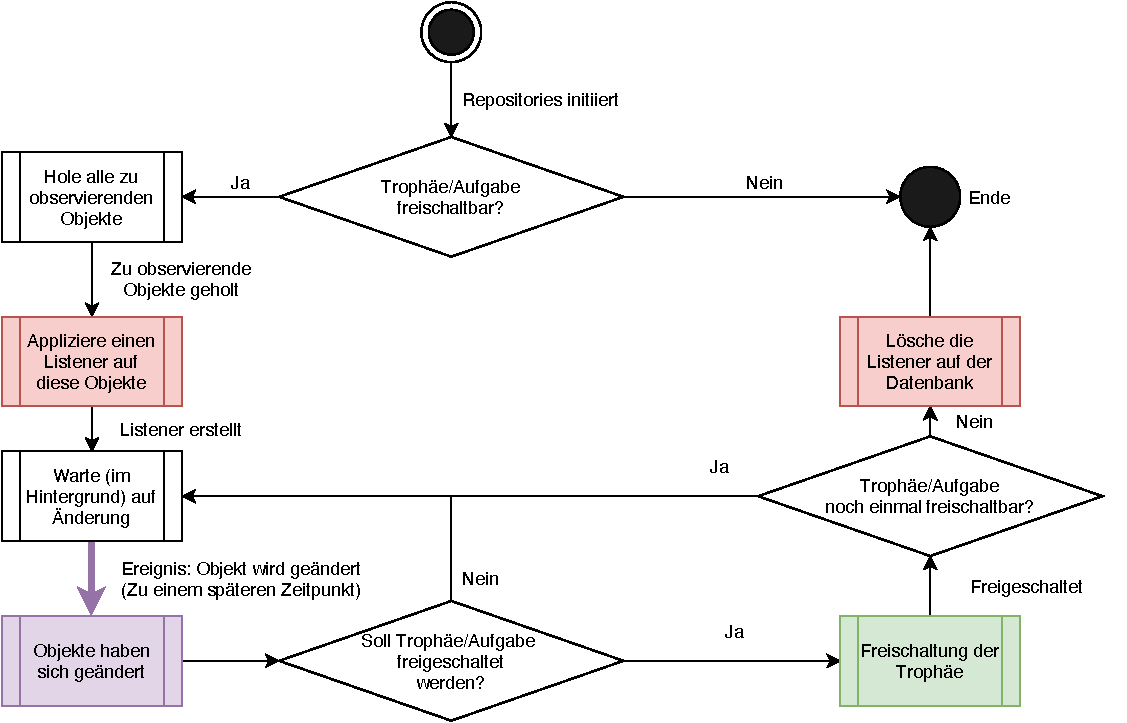
\includegraphics[width=\linewidth, bb=0 0 540 347]{daten-listener.pdf}
\caption{Ein Algorithmus für die Datenbank-Listener-basierte Freischaltung von Trophäen und Aufgaben. Rot hervorgehoben sind Prozesse, bei denen Listener appliziert oder entfernt werden. Violett hervorgehoben ist das auslösende Ereignis für eine Prüfung auf Freischaltung. Grün hervorgehoben ist die Freischaltung der Trophäe oder der Aufgabe.}\label{fig:daten-listener}
\end{figure}

\noindent Wie in \Cref{fig:daten-listener} illustriert, werden im Algorithmus bei einer Freischaltbarkeit der Trophäe bzw. Aufgabe die entsprechenden, zu observierenden Datenbankobjekte zunächst geholt. Wenn die Aufgabe oder die Trophäe bereits freigeschaltet wurde und nicht mehrmals freigeschaltet werden kann, werden keine Datenbank-Listener appliziert, um Ressourcen zu sparen. Wurden die zu observierenden Objekte geholt, wird ein Listener über das Repository-Interface der Datenbank auf diesen Objekten erstellt, welcher notifiziert wird, sobald die Datenbank eine Änderung der Objekte feststellt. Bei einer Änderung der relevanten Objekte, die im Hintergrund während der gesamten Laufzeit der App durch bestimmte Aktionen stattfinden kann, wird anschließend geprüft, ob die Trophäe oder Aufgabe freigeschaltet werden soll, oder nicht. Infolgedessen kann der Listener weiter fortexistieren, wenn bspw. die Trophäe oder die Aufgabe nicht freigeschaltet wurde oder mehrmals freigeschaltet werden können. Sonst wird der Listener vom Repository entfernt, um Ressourcen zu sparen, da er nicht weiter benötigt wird. Durch diesen Algorithmus konnten alle datenbasierten Errungenschaften implementiert werden. Beispielsweise existiert die Aufgabe \enquote{Spielregistrierung}, bei der ein Nutzer einen Spieler erstellen muss. Hierzu wird auf alle Objekte des \texttt{LocalPlayerRepository} ein Listener appliziert, und sobald ein Nutzer einen Spieler registriert und dieser im \texttt{LocalPlayerRepository} gespeichert wird, wird die Freischaltung der Aufgabe ausgelöst. Gleichzeitig lassen sich hierdurch QR-Code-basierte Aufgaben und Trophäen auch sehr leicht implementieren, indem die zu observierenden QR-Codes aus der Datenbank geholt werden, hierauf ein Listener erstellt wird, und beim Scannen eines neuen QR Codes geprüft wird, ob hierdurch die jeweilige Aufgabe oder Trophäe freigeschaltet werden soll.

\subsubsection{Implementation von interaktionsbasierten Errungenschaften}

Für bestimmte Aktionen, welche keine direkte Änderung von Objekten in der Datenbank induzieren, lässt sich der Algorithmus aus der vorigen Sektion nicht applizieren. Daher wurde hierfür ein weiterer Algorithmus entworfen:

\begin{figure}[H]
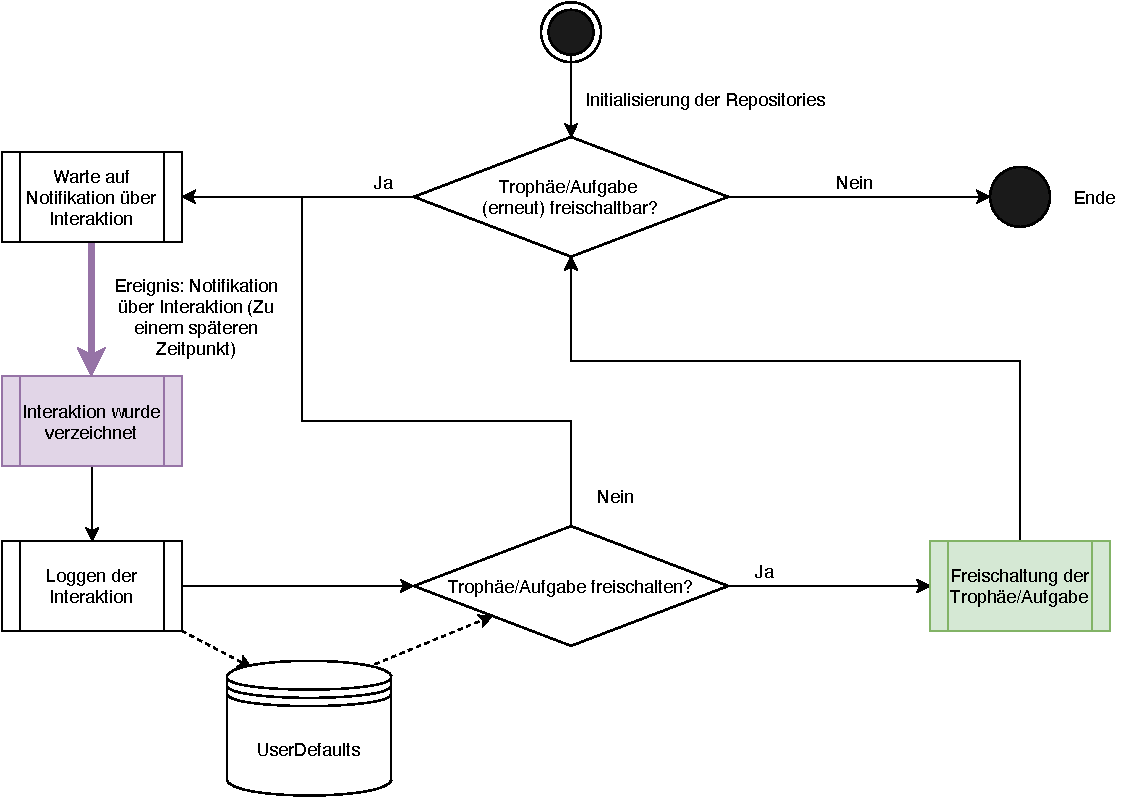
\includegraphics[width=\linewidth, bb=0 0 540 383]{interaktion-listener.pdf}
\caption{Ein Algorithmus für die interaktionsbasierte Freischaltung von Trophäen und Aufgaben. Violett hervorgehoben ist das auslösende Ereignis für eine Prüfung auf Freischaltung. Grün hervorgehoben ist die Freischaltung der Trophäe oder der Aufgabe.}\label{fig:interaktion-listener}
\end{figure}

\noindent Der in \Cref{fig:interaktion-listener} gezeigte Algorithmus ähnelt dem der datenbasierten Freischaltung, unterscheidet sich jedoch in wesentlichen Punkten. Statt Listener auf der Datenbank zu erstellen, wird eine Interaktion direkt aus dem UI an den Observer übergeben. Anschließend wird die Interaktion in den UserDefaults der App gespeichert, um anhand der vergangenen Interaktionen und der aktuellen Interaktion schließlich zu entscheiden, ob die Interaktion zu einer Freischaltung der jeweiligen Trophäe bzw. der jeweiligen Aufgabe führt. Beispielsweise existiert eine Trophäe \enquote{APP EXPLORER}, bei der die Besuche der 6 wichtigsten Ansichten als Interaktionen zwischengespeichert werden - wurden alle Ansichten besucht, wird die Trophäe freigeschaltet. Infolgedessen kann der Observer weiterhin bspw. von Besuchen neuer Ansichten informiert werden - durch die Freischaltung der nicht wiederholbaren Trophäe jedoch wird keine Prüfung auf Freischaltung mehr stattfinden, um Ressourcen zu sparen.

\subsubsection{Freischaltung und eventbasierte Darstellung der Freischaltungsansicht}

Sobald ein interaktions- oder datenbasierter Observer feststellt, dass eine Trophäe oder eine Aufgabe freigeschaltet werden soll, wird dies in der Datenbank persistiert (unter den Modellen \texttt{AchievedTrophy} und \texttt{CompletedTask}) und der Spieler erhält die damit verbundenen (Erfahrungs-)Punkte. Zuletzt wird die App über dieses Ereignis benachrichtigt, hierbei kommt ein in \Cref{ch:grundlagen} beschriebener eventbasierter Datenfluss zum Einsatz. Durch das Absenden des Events (beinhaltet Informationen über die Freischaltung) aus dem Hintergrundprozess der Freischaltung wird im Vordergrund die Darstellung einer Konfetti-Ansicht mit den entsprechenden Informationen ausgelöst.

\paragraph{Erweiterbarkeit und Änderbarkeit der Errungenschaften:} Durch die zuvor konzipierte Separation der Observer konnte deren Implementation hauptsächlich in generalisierten Oberklassen durchgeführt werden, um die konkrete Implementation der jeweiligen Freischaltungslogik der Trophäe oder Aufgabe so kompakt und robust wie möglich zu halten.

\paragraph{Testbarkeit:} Um die Implementation der Trophäen und Aufgaben besser testen zu können, wurde im QR-Code-Scanner (als Ausgangspunkt für verschiedene Trophäen und Aufgaben) zusätzlich eine Debug-Ansicht implementiert, mithilfe derer die verfügbaren QR Codes ausgewählt und ein Scannen simuliert werden kann.

\section{Integration des Crowd-Monitoring-Frameworks}

Zusätzlich zur Anbindung des Couchbase-Repository-Frameworks sollte auch die Reintegration der Crowd-Monitoring-Frameworks durchgeführt werden. Hierzu wurden die Komponenten, welche in der bestehenden Applikation zum Crowd-Monitoring-Framework gehörten, vom restlichen Teil der Applikation isoliert. Anschließend wurde das Crowd-Monitoring-Framework zu Testzwecken an die entwickelte UI der neuen Applikation angebunden. Hierzu mussten bestimmte Veränderungen und Bugfixes am Framework vorgenommen werden, damit das Framework kompiliert. Anschließend wurde getestet, inwiefern das Framework beim Aktivieren des Crowd-Monitorings innerhalb der App die entsprechenden Funktionalitäten weiterhin ausführt. Beim Testen konnte keine fehlerhafte Funktionsweise des Frameworks festgestellt werden, jedoch war die Testbarkeit des Frameworks eingeschränkt, da keine (für das Crowd-Monitoring benötigte) iBeacons vorhanden waren und Bluetooth auf dem iOS-Simulator nicht verfügbar ist. Während der Integration des Crowd-Monitoring-Frameworks wurden weitere technische Probleme, ähnlich zu den in \Cref{ch:einleitung} Beschriebenen, innerhalb des Frameworks identifiziert, beispielsweise der Zugriff auf einen nicht mehr verfügbaren Endpunkt und das Vorhandensein von Google Maps Schnittstellen und GeoJSON-Loadern, die in der neuen App durch die Repositories und MapBox ersetzt und bewusst vom Crowd-Monitoring-Framework separiert wurden. Günstigerweise wurde zu diesem Zeitpunkt eine Forschungsarbeit am Crowd-Monitoring-Framework durchgeführt bzw. sollte durchgeführt werden, so dass dem dazugehörigen Projektteam diese Probleme kommunziert werden konnten. Die Reimplementation und die Refaktorisierung des Crowd-Monitoring-Frameworks wird in diesem Rahmen außerhalb des Kontextes dieser Arbeit weiter durchgeführt. Um dies zu gewährleisten, wurde das Crowd-Monitoring-Framework in ein externes Pod-Repository (ähnlich zum Couchbase-Framework) ausgelagert und dort zur Weiterbearbeitung zur Verfügung gestellt. Außerdem wurden isolierte klare Schnittstellen vereinbart, über welche die Reintegration des Crowd-Monitoring-Frameworks mit sehr wenig Änderungs- bzw. Erweiterungsaufwand stattfinden kann.

\section{Dokumentation der Entwickler- und Distributionsleitfäden}

Zum Abschluss der Projektbearbeitung wurden außerdem noch ein Entwickler- und ein Distributionsleitfaden erarbeitet. Wesentlicher Bestandteil des Entwicklerleitfadens sind auch die technischen Erläuterungen des Konzeptes dieser Arbeit. Zukünftige Projektteams, die an der OUTPUT.DD-App weiter arbeiten, können über den Entwicklerleitfaden ein klares Verständnis der verwendeten Patterns und Strukturen erlangen, mit dem langfristigen Ziel, die Degradation der Codequalität und -struktur präventiv zu verhindern. Weitere Dokumente, wie die Auflistung aller Trophäen und Aufgaben, sowie derer Kriterien für die Freischaltung, sollen eine Hilfe darstellen, um die Konsistenz zwischen der iOS- und Android-Applikation zu gewährleisten. Im Distributionsleitfaden befinden sich weitere Beschreibungen, wie die CI-Pipeline für eine Distribution in einem iOS-Entwickler-Account genutzt werden kann.

  \chapter{Zusammenfassung}\label{ch:zusammenfassung}

Im Rahmen einer Projektbearbeitung im Sommersemester 2020 wurde ein Framework für Couchbase erstellt, welches das bestehende Realm-Framework in der OUTPUT.DD App ersetzen sollte. Bei der Erstellung wurden im Rahmen eines Audits zahlreiche, teils strukturelle oder architekturelle, Probleme und Antipatterns in der bestehenden OUTPUT.DD App identifiziert. Die Problemstellung dieser Arbeit war es somit, nicht nur das neue Datenbank-Framework in der OUTPUT.DD App zu integrieren, sondern auch einen allumfassenden Neuaufbau zu planen und durchzuführen. Hierdurch sollten die identifizierten Probleme behoben und verschiedene Strategien entworfen werden, mit denen das Wiedereintreten dieser Probleme verhindert werden soll.

\section{Vorgehensweise und Ergebnisse}

\noindent Hierzu wurden verschiedene Software-Patterns beschrieben, sowie deren Anwendungsbereiche und weshalb deren Nutzung einen signifikanten Vorteil für die Separabilität, Funktionalität und Erweiterbarkeit als zentrale Bestandteile der Codequalität bietet. Außerdem wurde die Struktur der bestehenden App anhand einer Dialoglandkarte analysiert und anschließend, mit Hinblick auf die Struktur des neuen Couchbase-Frameworks, in eine neue Top-Level-Architektur überführt, die eine Separation der unterschiedlichen Komponenten vorschlägt. Mithilfe konkreter Konzepte für die Strukturierung von Verzeichnissen anhand der horizontalen und vertikalen Teilung wurde die Neuimplementierung der iOS-App konzipiert und durchgeführt. Hierbei wurde als statisches Code-Analysetool SwiftLint eingeführt, welches zur Vermeidung von Code Smells beitragen soll. Begonnen wurde mit der Neuimplementation des Frontends auf Grundlage einer Modularisierung und Wiederverwendung von UI-Komponenten, sowie der Orientierung an Prinzipien der Usability und der OUTPUT.DD Corporate Identity. Hierbei wurden unter gemeinsamer Absprache bestimmte Teile der App auch optisch modernisiert und durch ein Dark-Mode-Feature ergänzt. Um den redundanten Arbeitsaufwand bei der Übermittlung der iOS-Applikation an App Store Connect zu reduzieren und gleichzeitig die iOS-Applikation über TestFlight testen zu können, wurde eine CI-Pipeline konzipiert, dokumentiert und auf GitHub integriert.

\begin{figure}[H]
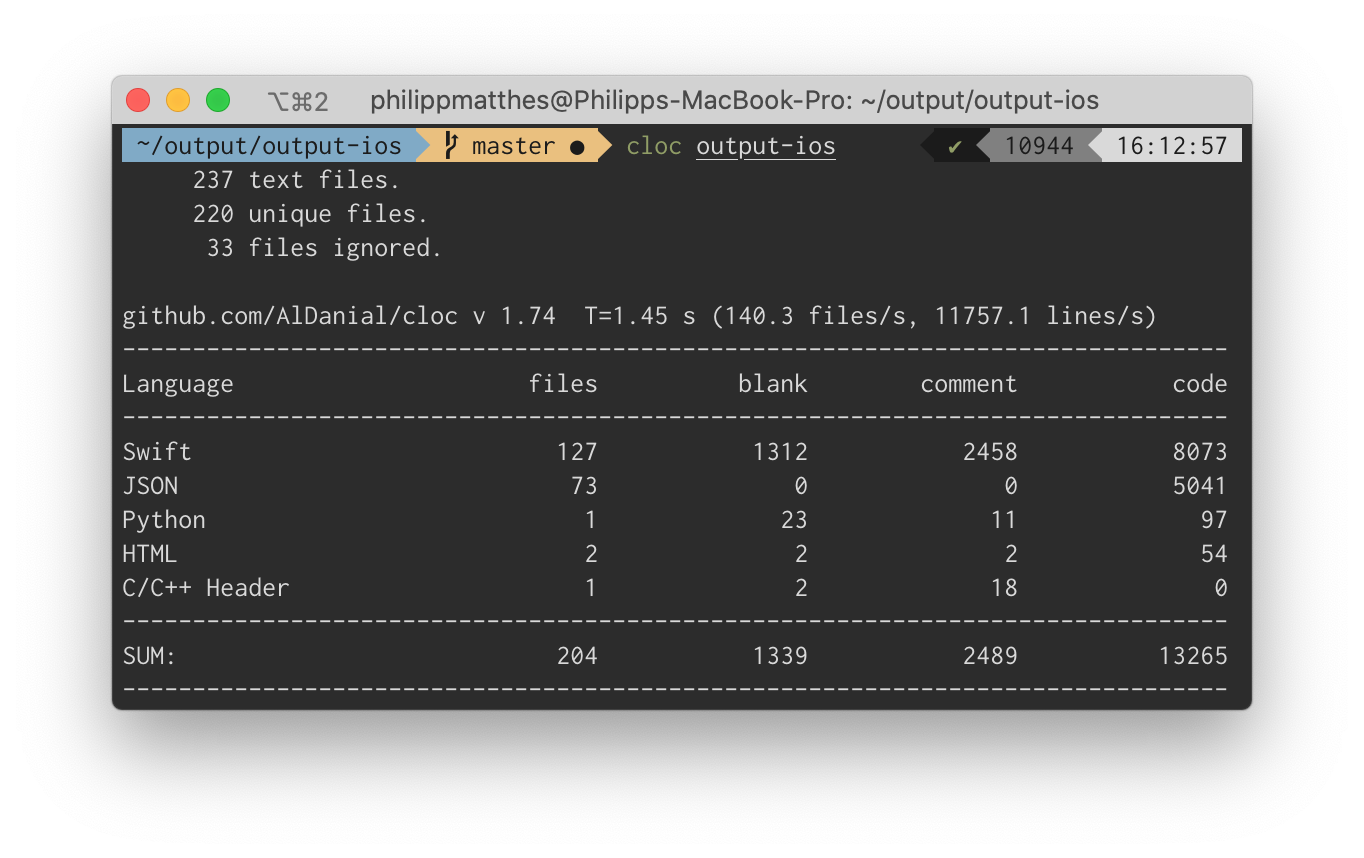
\includegraphics[width=\linewidth]{code.png}
\caption{Die neu implementierte App umfasst ca. 8000 Zeilen Swift Code.}\label{fig:code}
\end{figure}

\noindent Für die Integration des Datenbank-Backends wurden konkrete Patterns ausgewählt und verwendet, um gleichzeitig die Persistierung der Datenbankmodelle auf simulierten oder physischen Geräten und eine performante SwiftUI-Preview zu ermöglichen. Hierfür wurden insbesondere das Coordinator-Pattern, das Environment-Pattern, sowie das Proxy-Pattern verwendet. Durch die konsistente Nutzung dieser Architekturpattern konnte die Geschäftslogik der einzelnen Ansichten weiter voneinander separiert werden. Außerdem konnten die genannten Pattern genutzt werden, um zusätzlich zur lokalen Datenbank auch die Synchronisationskomponenten an diese anzubinden. Zum Testen der Datenbank- und Synchronisationsfunktionalitäten wurden konkrete Teststrategien angewandt, darunter die Generierung und Initialisierung von Daten zum Testen der Darstellung innerhalb der UI-Komponenten, sowie die Nutzung eines containerisierten Docker-Test-Setups für das Testen der Couchbase-Replikatoren. Abschließend wurden für die Implementation der Gamification-Errungenschaften konkrete Modelle und Basisalgorithmen entwickelt, mithilfe derer alle Errungenschaften weitestgehend unabhängig und separiert von den beteiligten UI-Komponenten implementiert werden konnten. Für die Fortführung des Projektes wurde diese Dokumentation neben weiteren Leitfäden mit besonders technischem Fokus erstellt, um als wesentlicher Teil des Entwicklerleitfadens zu dienen und zukünftig den Einstieg in die Entwicklung an der OUTPUT.DD App zu vereinfachen und zu vereinheitlichen.

\section{Offene Punkte}

Die Reimplementation der OUTPUT.DD App konnte vollständig durchgeführt werden und beinhaltet neben den bereits vorher existierenden Funktionalitäten, einer technischen, architekturellen und optischen Modernisierung auch allgemeine Verbesserungen in der Usability. Lediglich im Crowd-Monitoring-Framework konnten weitere Probleme identifiziert und kommuniziert werden, welche mithilfe klarer Integrationspunkte im Rahmen einer anderen Forschungsarbeit behoben werden sollen.

\noindent Bis zu OUTPUT.DD 2021 am 8. Juli 2021 wird die App weiterhin getestet und ggf. Verbesserungen und Optimierungen umgesetzt, welche sich aus dem Test-Feedback ergeben. Auch die Distribution der Apps und das Deployment des Couchbase-Backend auf einem Produktionssystem für OUTPUT.DD 2021 wird noch im Rahmen des Supportprozesses zukünftiger Teil dieser Arbeit sein.

\section{Danksagung}

Die Teilnahme an dieser Projektarbeit hat mir persönlich sehr viel Spaß gemacht und ich konnte meine Kenntnisse im Bereich Application Development weiter ausbauen. Ich danke meinem Betreuer, Dr. Thomas Springer, für das Vertrauen in meine Kompetenzen, mich mit einem sehr komplexen und vielseitigen Projekt wie diesem zu betrauen. Außerdem möchte ich B.-Sc. Felix Kästner danken für die sehr kompetente Unterstützung bei der Implementation und Lösungsfindung auf Android-Seite.


  \newpage

  % use lowercased roman page numbers for the appendix and the bibliography
  \pagenumbering{roman}

  % \printbibliography[heading=bibintoc]\label{sec:bibliography}%

  % \begin{appendices}
  %   \tocless\chapter{Appendix A}\label{appendix:a}

  % \end{appendices}

\end{document}
